\documentclass[aspectratio=169,10pt,t]{beamer}
\usepackage{issa}  % place issa.sty in the same folder
\definecolor{AccentCol}{HTML}{E05218}
\renewcommand{\lecnum}{1}
\newcommand{\evA}[3]{\fill[AccentCol](#1,0)circle(0.13);\draw[ISSAgrey](#1,0.13)--(#1,0.5);\node[anchor=south,text width=3.4cm,align=center,font=\fontsize{6}{7}\selectfont] at (#1,0.5){\textbf{\textcolor{AccentCol}{#2}}\\#3};}
\newcommand{\evB}[3]{\fill[AccentCol](#1,0)circle(0.13);\draw[ISSAgrey](#1,-0.13)--(#1,-0.5);\node[anchor=north,text width=3.4cm,align=center,font=\fontsize{6}{7}\selectfont] at (#1,-0.5){\textbf{\textcolor{AccentCol}{#2}}\\#3};}
\begin{document}
\titleslide{1}{Foundations, Paradigms,\\Defence Applications \& Data Pitfalls}{AI Foundations \textbullet\ ML Paradigms \textbullet\ Defence \& Wargaming Applications \textbullet\ Data Pitfalls}

%%%%%%%%%%%%%%%%%%%%%%%%% OVERVIEW %%%%%%%%%%%%%%%%%%%%%%%%%
\sect{Course Overview}
\begin{frame}{Course Overview --- 10-Lecture Roadmap (Unit 4: AI \& ML in Warfare)}
\subhead{Unit 4 Lecture Schedule: 10 Hours Total --- one story from data to autonomous decisions}
\figc{4.6cm}{\begin{tikzpicture}[x=3.05cm,y=-2.25cm]
\tikzset{L/.style={nd,text width=2.55cm,minimum height=1.55cm,inner sep=3pt,font=\fontsize{6.5}{8}\selectfont}}
\node[L,draw=AccentCol,fill=AccentCol!18,line width=1.4pt] (a) at (0,0) {\textbf{L1 \ \textcolor{AccentCol}{$\blacktriangleleft$ TODAY}}\\AI \& ML Foundations, Paradigms \& Data Pitfalls};
\node[L,fill=ISSAgrn!12,draw=ISSAgrn] (b) at (1,0) {\textbf{L2}\\Supervised Learning Part 1 --- Classification Algorithms for Defence};
\node[L,fill=violet!10,draw=violet] (c) at (2,0) {\textbf{L3}\\Supervised Learning Part 2 --- Regression, Sensor Fusion \& Practical Lab};
\node[L,fill=teal!12,draw=teal] (d) at (3,0) {\textbf{L4}\\Unsupervised Learning Part 1 --- Clustering \& Pattern Discovery};
\node[L,fill=ISSAred!10,draw=ISSAred] (e) at (4,0) {\textbf{L5}\\Unsupervised Learning Part 2 --- Anomaly Detection \& Cybersecurity};
\node[L,fill=blue!8,draw=blue!60!black] (f) at (0,1) {\textbf{L6}\\Reinforcement Learning Part 1 --- MDPs and Q-Learning};
\node[L,fill=green!10!teal!15,draw=teal!60!black] (g) at (1,1) {\textbf{L7}\\Reinforcement Learning Part 2 --- Policy Gradient Methods};
\node[L,fill=orange!12,draw=orange!70!black] (h) at (2,1) {\textbf{L8}\\RL Part 3 --- Multi-Agent Systems \& Autonomous Combat Platforms};
\node[L,fill=purple!10,draw=purple!70!black] (i) at (3,1) {\textbf{L9}\\Culmination \& Revision --- Integration Across All Modules};
\node[L,fill=yellow!20,draw=ISSAamb] (j) at (4,1) {\textbf{L10}\\Student Project Presentations \& Open Q\&A};
\foreach \u/\v in {a/b,b/c,c/d,d/e,f/g,g/h,h/i,i/j}{\draw[arr](\u)--(\v);}
\draw[arr](e.south)--++(0,-0.25)-|(f.north);
\node[lab,anchor=west] at (-0.45,-0.62) {Foundations + Supervised (L1--L3)};
\node[lab,anchor=west] at (2.55,-0.62) {Unsupervised (L4--L5)};
\node[lab,anchor=west] at (-0.45,1.62) {Reinforcement Learning (L6--L8)};
\node[lab,anchor=west] at (2.55,1.62) {Integration \& Assessment (L9--L10)};
\end{tikzpicture}}
\vspace{2pt}
\begin{ibox}\scriptsize\textbf{Reading the map:} L1 sets the vocabulary and the data-quality lens; L2--L3 teach prediction with labels; L4--L5 teach discovery without labels; L6--L8 teach decision-making by interaction; L9--L10 consolidate and assess.\end{ibox}
\end{frame}

\begin{frame}{Lecture 1 --- Structure, Format \& Learning Objectives}
\begin{columns}[T]
\column{0.50\textwidth}
\subhead{Lecture structure (45 min)}
\figc{1.5cm}{\begin{tikzpicture}[x=0.19cm]
\fill[ISSAblue!70] (0,0) rectangle (5,0.7);\fill[AccentCol] (5,0) rectangle (35,0.7);\fill[ISSAgrn] (35,0) rectangle (45,0.7);
\node[white,font=\tiny] at (2.5,0.35){5};\node[white,font=\tiny] at (20,0.35){30 min core lecture};\node[white,font=\tiny] at (40,0.35){10};
\node[lab] at (2.5,-0.35){Q\&A};\node[lab] at (20,-0.35){Core lecture content (this deck)};\node[lab] at (40,-0.35){Auto-quiz};
\end{tikzpicture}}
\begin{tl}\item \textbf{5 min} --- Q\&A on previous session
\item \textbf{30 min} --- core lecture content (this deck)
\item \textbf{10 min} --- auto-quiz (15 questions $\times$ 40 s)
\item Format: 4-pane layout, equations, defence examples\end{tl}
\begin{ibox}\scriptsize\textbf{DATA PITFALLS} thread woven throughout --- a critical lens for every AI/ML practitioner in Defence Research. Based on AK Dhamija (SlideShare: Goody Research) plus established ML literature.\end{ibox}
\begin{cbox}[ISSAnavy]{Parts of each lecture}\scriptsize
\textbf{Part 1:} lecture slides \ \textbf{Part 2:} auto-quiz (40 s/Q)\\\textbf{Part 3:} quiz answers + assignment solutions \ \textbf{Part 4:} instructor manual\end{cbox}
\column{0.48\textwidth}
\subhead{Learning objectives}
\begin{cbox}{By the end of this lecture you can\ldots}
\begin{te}
\item Define AI, ML and core paradigms precisely
\item Trace evolution: Classical AI $\to$ GenAI
\item Distinguish the 5 ML learning paradigms
\item Describe Deep Learning key architectures
\item Explain LLMs and RAG in defence context
\item Map AI/ML to Defence \& Wargaming use cases
\item Spot flaws in data analysis \& interpretation (Simpson, $H_0$, correlation vs causation)
\item Identify and avoid 6 critical data pitfalls
\end{te}\end{cbox}
\begin{rbox}\scriptsize\textbf{Anchor:} all numerical examples \& case studies are anchored in Defence R\&D and Wargaming Simulation contexts.\end{rbox}
\begin{cbox}[ISSAblue]{Syllabus --- Unit 4}\scriptsize AI \& ML Paradigms $\mid$ Supervised Learning for Defence $\mid$ Unsupervised Learning \& Clustering $\mid$ RL for Autonomous Systems\end{cbox}
\end{columns}
\end{frame}


%%%%%%%%%%%%%%%%%%%%%%%%% 0. DATA CAN LIE %%%%%%%%%%%%%%%%%%%%%%%%%
\sect{0. Data Can Lie}
\begin{frame}{Before Any Algorithm: Data Can Lie --- Six Famous Failures, Six Disciplines}
\subhead{Every one of these errors has a twin in defence analysis and wargaming}
\figc{5.2cm}{\begin{tikzpicture}
\tikzset{G/.style={nd,text width=4.75cm,align=left,minimum height=2.3cm,font=\fontsize{7}{8.3}\selectfont,inner sep=3pt}}
\node[G,draw=ISSAblue,fill=ISSAblue!7]at(-5.0,1.25){\textbf{\textcolor{ISSAblue}{AERONAUTICS --- 1943}}\\Engineers wanted to armour where returning bombers had bullet holes. Wald: armour where they had \emph{none}.\\\textbf{Error:} survivorship bias.\\\textbf{Wargame twin:} learning only from won engagements.};
\node[G,draw=ISSAred,fill=ISSAred!6]at(0,1.25){\textbf{\textcolor{ISSAred}{ENGINEERING --- 1986}}\\Challenger O-ring analysis looked only at flights \emph{with} damage; the 17 damage-free warm-weather flights were left out --- hiding the temperature trend.\\\textbf{Error:} missing / selected data.\\\textbf{Twin:} dropping ``no-event'' sorties.};
\node[G,draw=violet,fill=violet!7]at(5.0,1.25){\textbf{\textcolor{violet}{PSYCHOLOGY --- 1960s}}\\Israeli Air Force instructors: praise after good landings was followed by worse ones; criticism by better ones. Truth: regression to the mean.\\\textbf{Error:} attributing chance to cause.\\\textbf{Twin:} ``retraining fixed the worst units''.};
\node[G,draw=ISSAgrn,fill=ISSAgrn!7]at(-5.0,-1.25){\textbf{\textcolor{ISSAgrn}{BIOLOGY / MEDICINE --- 1990s}}\\A pneumonia-risk model learned that asthma \emph{lowers} death risk --- because asthmatics were sent straight to intensive care.\\\textbf{Error:} confounding by treatment.\\\textbf{Twin:} ``units under air cover take more losses''.};
\node[G,draw=ISSAamb,fill=ISSAyell!45]at(0,-1.25){\textbf{\textcolor{ISSAamb!80!black}{STATISTICS --- 1973 / 1986}}\\Berkeley admissions and kidney-stone trials: a treatment or group that wins in \emph{every} subgroup loses in the total.\\\textbf{Error:} Simpson's paradox.\\\textbf{Twin:} ``AI-equipped units win less''.};
\node[G,draw=AccentCol,fill=AccentCol!8]at(5.0,-1.25){\textbf{\textcolor{AccentCol}{DEFENCE --- 1988 / 2003}}\\USS Vincennes downed an airliner the crew believed was attacking; Patriot batteries engaged two friendly aircraft. Data and automation were trusted over doubt.\\\textbf{Error:} expectation \& automation bias.\\\textbf{Twin:} rubber-stamping AI alerts.};
\end{tikzpicture}}
\begin{wbox}\scriptsize\textbf{The point of this section:} algorithms do not fix these errors --- they \emph{automate} and \emph{scale} them. Before we learn a single model, we learn how data and interpretation fail.\end{wbox}
\end{frame}

\begin{frame}{Simpson's Paradox (I) --- Never Add or Average Percentages: Use the Counts}
\subhead{Kidney-stone treatments (Charig et al., \textit{BMJ}, 1986): A = open surgery, B = percutaneous nephrolithotomy}
\begin{columns}[T]
\column{0.56\textwidth}
\figc{2.6cm}{\small\renewcommand{\arraystretch}{1.25}\begin{tabular}{lcc}\toprule\textbf{Stone size}&\textbf{Treatment A}&\textbf{Treatment B}\\\midrule Small stones&\cellcolor{ISSAgrn!25}\textbf{81 / 87 = 93\%}&234 / 270 = 87\%\\Large stones&\cellcolor{ISSAgrn!25}\textbf{192 / 263 = 73\%}&55 / 80 = 69\%\\\midrule\textbf{Combined}&273 / 350 = \textbf{78\%}&\cellcolor{ISSAgrn!25}289 / 350 = \textbf{83\%}\\\bottomrule\end{tabular}}
\sm{Cells show successes / patients = success rate. A wins in BOTH subgroups yet loses overall.}
\begin{wbox}\scriptsize\textbf{Tempting mistake:} adding percentages ($93+73=166$ vs $87+69=156$) or averaging them (83\% vs 78\%) --- meaningless: it ignores group sizes.\end{wbox}
\begin{fbx}{Combined rate = weighted average by group size}\[\text{A: }\tfrac{87(0.93)+263(0.73)}{350}=\tfrac{81+192}{350}=78\%\]\[\text{B: }\tfrac{270(0.87)+80(0.69)}{350}=\tfrac{234+55}{350}=83\%\]\end{fbx}
\column{0.42\textwidth}
\subhead{Why: case mix differs between treatments}
\figc{1.6cm}{\begin{tikzpicture}[x=0.06cm]
\fill[ISSAgrn!55](0,0.9)rectangle(24.9,1.5);\fill[ISSAred!60](24.9,0.9)rectangle(100,1.5);\node[anchor=east,font=\scriptsize\bfseries]at(-1,1.2){A};\node[font=\tiny]at(12.4,1.2){87 small};\node[font=\tiny,white]at(62,1.2){263 large (75\%) --- the HARD cases};
\fill[ISSAgrn!55](0,0)rectangle(77.1,0.6);\fill[ISSAred!60](77.1,0)rectangle(100,0.6);\node[anchor=east,font=\scriptsize\bfseries]at(-1,0.3){B};\node[font=\tiny]at(38,0.3){270 small (77\%) --- the EASY cases};\node[font=\tiny,white]at(88.5,0.3){80 large};
\end{tikzpicture}}
\begin{tl}\item Large stones are harder to treat \emph{and} were mostly given treatment A\item So A's total is dragged down by case mix, not by worse treatment\item \textbf{Confounder:} stone size (severity) drives both the choice of treatment and the outcome\end{tl}
\begin{rbox}\scriptsize\textbf{Rule:} always compute totals from raw counts, show the counts beside every percentage, and stratify by the variables that drive both assignment and outcome.\end{rbox}
\end{columns}
\end{frame}

\begin{frame}{Simpson's Paradox (II) --- The Wargaming Twin: ``AI-Assisted Units Perform Worse''?}
\subhead{Exercise records: engagements won / fought, split by terrain (illustrative teaching data)}
\begin{columns}[T]
\column{0.54\textwidth}
\figc{2.4cm}{\small\renewcommand{\arraystretch}{1.25}\begin{tabular}{lcc}\toprule\textbf{Terrain}&\textbf{AI-assisted units}&\textbf{Conventional units}\\\midrule Open / easy&\cellcolor{ISSAgrn!25}\textbf{81 / 90 = 90\%}&238 / 280 = 85\%\\Mountain / hard&\cellcolor{ISSAgrn!25}\textbf{105 / 210 = 50\%}&18 / 40 = 45\%\\\midrule\textbf{All terrain}&186 / 300 = \textbf{62\%}&\cellcolor{ISSAred!20}256 / 320 = \textbf{80\%}\\\bottomrule\end{tabular}}
\figc{2.4cm}{\begin{tikzpicture}\begin{axis}[ybar,width=7.4cm,height=3.2cm,symbolic x coords={Open,Mountain,All terrain},xtick=data,ymin=0,ymax=105,bar width=12pt,enlarge x limits=0.25,legend style={at={(0.5,1.03)},anchor=south,legend columns=2},nodes near coords,nodes near coords style={font=\fontsize{5.5}{6}\selectfont},ylabel={win rate (\%)},ymajorgrids]
\addplot[fill=AccentCol!80]coordinates{(Open,90)(Mountain,50)(All terrain,62)};\addlegendentry{AI-assisted}
\addplot[fill=ISSAgrey!70]coordinates{(Open,85)(Mountain,45)(All terrain,80)};\addlegendentry{Conventional}
\end{axis}\end{tikzpicture}}
\column{0.44\textwidth}
\begin{wbox}\scriptsize\textbf{Headline a staff officer might write:} ``AI-assisted units win only 62\% vs 80\% --- withdraw the AI tool.''\end{wbox}
\begin{rbox}\scriptsize\textbf{The truth:} AI-assisted units win MORE in every terrain (+5 points in both). They were deliberately sent to the hard mountain sectors: 210 of their 300 engagements (70\%) vs 40 of 320 (12.5\%) for conventional units.\end{rbox}
\begin{cbox}[ISSAnavy]{Same pattern, real world: UC Berkeley 1973}\scriptsize Overall admission: men 44\%, women 35\%. Department by department there was no bias against women --- women applied more to the most competitive departments (Bickel, Hammel \& O'Connell, \textit{Science}, 1975).\end{cbox}
\begin{ibox}\scriptsize\textbf{Ask every time:} what decided which units, patients or sorties ended up in each group? That variable must be stratified or controlled.\end{ibox}
\end{columns}
\end{frame}

\begin{frame}{The Null Hypothesis \& Statistical Significance --- What a p-value Says}
\begin{columns}[T]
\column{0.50\textwidth}
\figc{2.7cm}{\begin{tikzpicture}\begin{axis}[width=7.0cm,height=3.4cm,domain=-3.5:6,samples=80,ticks=none,xlabel={test statistic},ymin=0,legend pos=north east]
\addplot[fill=ISSAred!35,draw=none,domain=1.96:3.5]{exp(-x^2/2)/2.5066}\closedcycle;
\addplot[fill=ISSAamb!40,draw=none,domain=-1:1.96]{exp(-(x-2.5)^2/2)/2.5066}\closedcycle;
\addplot[ISSAblue,thick]{exp(-x^2/2)/2.5066};\addplot[ISSAgrn,thick]{exp(-(x-2.5)^2/2)/2.5066};
\draw[dashed](axis cs:1.96,0)--(axis cs:1.96,0.43);
\node[font=\tiny,ISSAblue]at(axis cs:-1.5,0.36){$H_0$: no effect};\node[font=\tiny,ISSAgrn]at(axis cs:4.3,0.36){$H_1$: real effect};
\node[font=\tiny,ISSAred]at(axis cs:2.75,0.03){$\alpha$};\node[font=\tiny,ISSAamb!70!black]at(axis cs:1.4,0.05){$\beta$};\node[font=\tiny,anchor=south west]at(axis cs:1.98,0.40){critical value};
\end{axis}\end{tikzpicture}}
\figc{1.55cm}{\scriptsize\renewcommand{\arraystretch}{1.15}\begin{tabular}{lcc}\toprule&$H_0$ true (no effect)&$H_0$ false (real effect)\\\midrule Reject $H_0$&\cellcolor{ISSAred!20}Type I error ($\alpha$): false alarm&Correct (power $=1-\beta$)\\Keep $H_0$&Correct&\cellcolor{ISSAamb!30}Type II error ($\beta$): missed effect\\\bottomrule\end{tabular}}
\begin{ibox}\scriptsize\textbf{p-value} = probability of data at least this extreme \emph{if $H_0$ were true}. It is NOT the probability that $H_0$ is true, and NOT the size or importance of the effect.\end{ibox}
\column{0.48\textwidth}
\begin{cbox}[ISSAnavy]{Defence example: radar-absorbent coating trial (illustrative)}\scriptsize $H_0$: the new coating does not change detection probability. 40 sorties each: baseline detected \textbf{26/40 (65\%)}, new coating \textbf{18/40 (45\%)}.\end{cbox}
\begin{fbx}{Two-proportion z-test}\[\hat p=\tfrac{44}{80}=0.55\]\[SE=\sqrt{0.55(0.45)\big(\tfrac1{40}+\tfrac1{40}\big)}=0.111\]\[z=\frac{0.65-0.45}{0.111}=1.80\ \Rightarrow\ p\approx0.072\ \ (>0.05)\]\end{fbx}
\begin{wbox}\scriptsize\textbf{Wrong conclusion:} ``the coating doesn't work''. A 20-point drop is large; the trial was under-powered. \textbf{Absence of evidence $\neq$ evidence of absence.} Power calculation: detecting 65\%$\to$45\% with 80\% power at $\alpha=0.05$ needs $\approx\mathbf{93}$ sorties per arm, not 40.\end{wbox}
\end{columns}
\end{frame}

\begin{frame}{Statistical vs Practical Significance --- and the p-hacking Trap}
\begin{columns}[T]
\column{0.50\textwidth}
\subhead{``Significant'' is not ``important''}
\begin{cbox}[ISSAnavy]{Huge sample, trivial effect (illustrative)}\scriptsize 1,000,000 simulated engagements per variant: hit rate 50.0\% vs 50.2\%. $SE=\sqrt{0.25\cdot2/10^6}=0.0007$, $z=0.002/0.0007\approx2.8$, $p\approx0.005$: ``highly significant'' --- yet 0.2 points will never change a tactical decision.\end{cbox}
\begin{cbox}[ISSAgrn]{Report what matters}\scriptsize Effect size (difference, ratio, Cohen's $d$) with a \textbf{95\% confidence interval}, and the cost/benefit of acting on it. A wide CI that includes zero \emph{and} large effects means ``we don't know yet'' --- collect more data.\end{cbox}
\begin{cbox}[violet]{Psychology's warning: the replication crisis}\scriptsize When 100 published psychology studies were repeated, only about 36\% gave a significant result again (Open Science Collaboration, \textit{Science}, 2015). Small samples + flexible analysis + publication of ``significant'' results only.\end{cbox}
\column{0.48\textwidth}
\subhead{Run enough tests and something will be ``significant''}
\figc{2.6cm}{\begin{tikzpicture}\begin{axis}[width=6.6cm,height=3.3cm,xlabel={number of independent tests $m$ (all with no real effect)},ylabel={P(at least one $p<0.05$)},xmin=1,xmax=40,ymin=0,ymax=1,domain=1:40,samples=40,ymajorgrids]
\addplot[AccentCol,thick]{1-0.95^x};\fill[ISSAred](axis cs:20,0.642)circle(1.6pt);\node[font=\tiny,ISSAred,anchor=north west]at(axis cs:20.5,0.62){$m=20$: 64\%};
\end{axis}\end{tikzpicture}}
\begin{fbx}{Family-wise error and Bonferroni correction}\[P(\ge1\text{ false positive})=1-(1-\alpha)^{m}\]\[\text{Bonferroni: }\alpha_{\text{per test}}=\alpha/m\]\end{fbx}
\begin{wbox}\scriptsize\textbf{Wargame trap:} testing 20 tactics, sectors or time windows and reporting the one with $p<0.05$ is p-hacking. Pre-register the hypothesis, correct for multiple tests, and confirm on fresh exercise data.\end{wbox}
\end{columns}
\end{frame}

\begin{frame}{Linear Correlation --- One Number Cannot Describe a Relationship}
\begin{columns}[T]
\column{0.58\textwidth}
\subhead{Anscombe's quartet (statistics, 1973): four datasets, identical summary statistics}
\figc{2.45cm}{\begin{tikzpicture}[x=0.16cm,y=0.16cm]
\foreach \sx/\sy/\lbl in {0/0/I linear,19/0/II curved,0/-14/III one outlier,19/-14/IV one leverage point}{\begin{scope}[shift={(\sx,\sy)}]\draw[ISSAgrey](3,2)rectangle(20,13.5);\draw[AccentCol,thick](3,4.5)--(20,13);\node[font=\fontsize{5.5}{6}\selectfont\bfseries,anchor=north west]at(3.2,13.4){\lbl};\end{scope}}
\foreach \x/\y in {10/8.04,8/6.95,13/7.58,9/8.81,11/8.33,14/9.96,6/7.24,4/4.26,12/10.84,7/4.82,5/5.68}{\node[pt1]at(\x,\y){};}
\foreach \x/\y in {10/9.14,8/8.14,13/8.74,9/8.77,11/9.26,14/8.10,6/6.13,4/3.10,12/9.13,7/7.26,5/4.74}{\node[pt1]at(\x+19,\y){};}
\foreach \x/\y in {10/7.46,8/6.77,13/12.74,9/7.11,11/7.81,14/8.84,6/6.08,4/5.39,12/8.15,7/6.42,5/5.73}{\node[pt1]at(\x,\y-14){};}
\foreach \x/\y in {8/6.58,8/5.76,8/7.71,8/8.84,8/8.47,8/7.04,8/5.25,19/12.50,8/5.56,8/7.91,8/6.89}{\node[pt1]at(\x+19,\y-14){};}
\end{tikzpicture}}
\sm{All four: mean $x=9$, mean $y=7.50$, variances equal, $r=0.816$, fitted line $y=3.00+0.500x$.}
\begin{rbox}\scriptsize\textbf{Rule:} \emph{plot} the data before trusting $r$, a regression line or an AI feature-importance score.\end{rbox}
\column{0.40\textwidth}
\begin{fbx}{Pearson correlation}\[r=\frac{\sum(x_i-\bar x)(y_i-\bar y)}{\sqrt{\sum(x_i-\bar x)^2\sum(y_i-\bar y)^2}}\in[-1,1]\]\end{fbx}
\begin{tl}\item $r$ measures only \textbf{linear} association; it is driven by outliers and leverage points\item $r^2$ = share of variance explained by the straight line\end{tl}
\subhead{Aeronautics: $r\approx0$, yet perfect dependence}
\figc{1.5cm}{\begin{tikzpicture}\begin{axis}[width=5.6cm,height=2.6cm,xlabel={airspeed},ylabel={total drag},ticks=none,domain=0.4:3,samples=40]
\addplot[AccentCol,thick]{0.5/x^2+0.25*x^2};\addplot[ISSAblue,dashed]{0.1+0.6/x^2};\addplot[ISSAred,dashed]{0.2*x^2};
\end{axis}\end{tikzpicture}}
\sm{Induced drag falls and parasite drag rises with speed: the U-shaped total has near-zero linear $r$ over the envelope.}
\end{columns}
\end{frame}

\begin{frame}{Correlation $\neq$ Causation --- Spurious Correlation and How It Arises}
\figc{2.1cm}{\begin{tikzpicture}
\tikzset{V/.style={circle,draw=ISSAnavy,fill=ISSAlblue!45,inner sep=1.5pt,minimum size=0.6cm,font=\scriptsize}}
\begin{scope}\node[V](x)at(0,0){$X$};\node[V](y)at(1.8,0){$Y$};\node[V,fill=ISSAyell](z)at(0.9,1.1){$Z$};\draw[arr](z)--(x);\draw[arr](z)--(y);\draw[dashed,ISSAred,<->](x)--(y);\node[lab]at(0.9,-0.65){\textbf{confounder}};\end{scope}
\begin{scope}[xshift=3.6cm]\node[V](x)at(0,0){$X$};\node[V](y)at(1.8,0){$Y$};\draw[arr](y)--(x);\node[lab]at(0.9,-0.65){\textbf{reverse causation}};\end{scope}
\begin{scope}[xshift=7.2cm]\node[V](x)at(0,0){$X$};\node[V](y)at(1.8,0){$Y$};\node[V,fill=ISSAred!25](s)at(0.9,1.1){$S$};\draw[arr](x)--(s);\draw[arr](y)--(s);\node[lab]at(0.9,-0.65){\textbf{selection on $S$}};\end{scope}
\begin{scope}[xshift=10.8cm]\node[V](x)at(0,0){$X$};\node[V](y)at(1.8,0){$Y$};\node[font=\scriptsize]at(0.9,0.75){?};\node[lab]at(0.9,-0.65){\textbf{pure chance (data dredging)}};\end{scope}
\end{tikzpicture}}
\begin{columns}[T]
\column{0.50\textwidth}
\begin{cbox}[ISSAamb]{Statistics / biology}\scriptsize \textbf{Storks and babies:} across 17 European countries, stork pairs correlate with birth rate ($r\approx0.62$, Matthews 2000). Confounder: land area and rural population. \textbf{Ice-cream sales and drownings:} both driven by summer heat.\end{cbox}
\begin{cbox}[ISSAred]{Engineering --- reverse causation}\scriptsize Vehicles with the most maintenance hours have the most breakdowns. Maintenance does not cause failure: failing vehicles \emph{attract} maintenance.\end{cbox}
\column{0.48\textwidth}
\begin{cbox}[AccentCol]{Defence \& wargaming}\scriptsize \textbf{Confounder:} ``catering-quality score'' vs exercise win rate, $r=0.71$; controlling for unit budget/readiness, $r_{\text{partial}}=0.09$ ($p=0.42$). \textbf{Selection:} analysing only engagements that were reported upward.\end{cbox}
\begin{cbox}[ISSAnavy]{Data dredging}\scriptsize Screen 1,000 candidate indicators with no real effect at $\alpha=0.05$: expect $\approx$\textbf{50} ``significant'' correlations by chance alone. AI feature-mining does exactly this at scale.\end{cbox}
\begin{rbox}\scriptsize\textbf{To claim causation:} a controlled experiment (randomised trial, A/B wargame), or a causal design that blocks confounders --- plus a plausible mechanism.\end{rbox}
\end{columns}
\end{frame}

\begin{frame}{Regression to the Mean --- When Chance Masquerades as Cause}
\begin{columns}[T]
\column{0.50\textwidth}
\figc{3.2cm}{\begin{tikzpicture}\begin{axis}[width=6.8cm,height=3.9cm,xlabel={performance on exercise 1},ylabel={performance on exercise 2},xmin=40,xmax=100,ymin=40,ymax=100,ymajorgrids]
\addplot[only marks,mark=*,mark size=1pt,ISSAblue!70]coordinates{(48,62)(52,58)(55,66)(58,61)(60,70)(62,64)(64,72)(66,67)(68,69)(70,74)(70,65)(72,71)(74,73)(76,70)(78,77)(80,74)(82,79)(85,76)(88,80)(92,78)(55,60)(65,71)(75,68)(85,82)(90,76)};
\addplot[ISSAgrey,dashed,domain=40:100]{x};\addplot[AccentCol,thick,domain=40:100]{0.5*x+35};
\node[font=\tiny,anchor=west]at(axis cs:41,46){$y=x$ (no regression)};\node[font=\tiny,AccentCol,anchor=west]at(axis cs:76,92){best fit: slope $<1$};
\end{axis}\end{tikzpicture}}
\sm{Illustrative data. Whenever luck contributes to a score, extreme scorers move toward the average next time --- with no intervention at all.}
\column{0.48\textwidth}
\begin{cbox}[violet]{Psychology + aeronautics: Israeli Air Force flight school}\scriptsize Instructors observed that praise after an excellent landing was usually followed by a worse one, and criticism after a bad landing by a better one --- and concluded that punishment works. Kahneman showed it was regression to the mean: an exceptional landing is partly luck.\end{cbox}
\begin{cbox}[ISSAgrn]{Biology: where the word comes from}\scriptsize Galton (1886): children of very tall parents are tall, but less extreme --- ``regression towards mediocrity''. The statistical term ``regression'' (Lecture 3) is named after this effect.\end{cbox}
\begin{wbox}\scriptsize\textbf{Defence trap:} ``the five worst-scoring battalions improved after the new AI training aid''. They would have improved anyway. \textbf{Fix:} compare against a control group of equally poor units that did not get the intervention.\end{wbox}
\end{columns}
\end{frame}

\begin{frame}{The Base-Rate Fallacy --- Why a ``99\% Accurate'' Detector Mostly Cries Wolf}
\begin{columns}[T]
\column{0.54\textwidth}
\subhead{10,000 air tracks; 10 are real threats (base rate 0.1\%)}
\figc{3.3cm}{\begin{tikzpicture}[level distance=1.3cm]
\node[ndN,minimum width=2.2cm](a)at(0,0){10,000 tracks};
\node[ndR,minimum width=2.0cm](t)at(-2.6,-1.4){10 threats};\node[ndG,minimum width=2.0cm](n)at(2.6,-1.4){9,990 non-threats};
\node[ndR,minimum width=1.7cm](tp)at(-3.6,-2.9){$\approx$10 alarms\\\sm{(99\% sensitivity)}};\node[nd,minimum width=1.4cm](fn)at(-1.6,-2.9){0.1 missed};
\node[ndY,minimum width=1.9cm](fp)at(1.5,-2.9){$\approx$100 false alarms\\\sm{(1\% of 9,990)}};\node[nd,minimum width=1.6cm](tn)at(3.9,-2.9){9,890 cleared};
\draw[arr](a)--(t);\draw[arr](a)--(n);\draw[arr](t)--(tp);\draw[arr](t)--(fn);\draw[arr](n)--(fp);\draw[arr](n)--(tn);
\end{tikzpicture}}
\begin{fbx}{Bayes' theorem: positive predictive value}\[P(\text{threat}\mid\text{alarm})=\frac{0.99\times0.001}{0.99\times0.001+0.01\times0.999}\approx\frac{10}{110}\approx\mathbf{9\%}\]\end{fbx}
\column{0.44\textwidth}
\begin{cbox}[ISSAgrn]{Biology / medicine}\scriptsize A screening test with 99\% sensitivity and 99\% specificity for a disease with 1\% prevalence: only \textbf{50\%} of positives are truly ill. Doctors routinely over-estimate this figure.\end{cbox}
\begin{wbox}\scriptsize\textbf{Defence consequence:} 10 of every 11 IADS alarms are false. Operators learn to distrust the system (alarm fatigue) --- or engage everything. Either way the ``99\% accuracy'' brochure figure misleads.\end{wbox}
\begin{rbox}\scriptsize\textbf{Always ask:} what is the base rate in the \emph{deployment} stream? Report precision (PPV) at that base rate, and design a second-stage check (human or sensor) for alarms.\end{rbox}
\end{columns}
\end{frame}

\begin{frame}{Engineering Lesson: Challenger (1986) --- The Data You Leave Out}
\begin{columns}[T]
\column{0.50\textwidth}
\subhead{What was examined: only flights with O-ring damage}
\figc{2.05cm}{\begin{tikzpicture}\begin{axis}[width=6.6cm,height=3.2cm,xlabel={launch temperature ($^\circ$F)},ylabel={damage incidents},xmin=25,xmax=85,ymin=-0.3,ymax=3.6,ymajorgrids]
\addplot[only marks,mark=*,mark size=1.6pt,ISSAred]coordinates{(53,3)(57,1)(58,1)(63,1)(70,1)(70,1)(75,2)};
\node[font=\tiny,anchor=north]at(axis cs:55,-0.05){no obvious trend};
\end{axis}\end{tikzpicture}}
\subhead{All flights: damage-free flights included}
\figc{2.05cm}{\begin{tikzpicture}\begin{axis}[width=6.6cm,height=3.2cm,xlabel={launch temperature ($^\circ$F)},ylabel={damage incidents},xmin=25,xmax=85,ymin=-0.3,ymax=3.6,ymajorgrids]
\addplot[only marks,mark=*,mark size=1.6pt,ISSAred]coordinates{(53,3)(57,1)(58,1)(63,1)(70,1)(70,1)(75,2)};
\addplot[only marks,mark=o,mark size=1.6pt,ISSAblue]coordinates{(66,0)(67,0)(67.3,0)(67.6,0)(68,0)(69,0)(70.3,0)(70.6,0)(72,0)(73,0)(75.3,0)(76,0)(76.3,0)(78,0)(79,0)(81,0)};
\draw[dashed,ISSAred,thick](axis cs:31,-0.3)--(axis cs:31,3.6);\node[font=\tiny,ISSAred,anchor=west]at(axis cs:31.5,3.2){launch day forecast: 31$^\circ$F};
\end{axis}\end{tikzpicture}}
\sm{Approximate reconstruction of the pre-launch flight record (cf. Dalal, Fowlkes \& Hoadley, \textit{JASA}, 1989).}
\column{0.48\textwidth}
\begin{cbox}[ISSAred]{What happened}\scriptsize On the eve of launch, engineers and managers reviewed O-ring damage against temperature using mainly the flights that \emph{had} damage. The picture looked flat. Every flight below 66$^\circ$F had damage. Challenger launched at about 31$^\circ$F --- far colder than any previous flight --- and was lost with its crew of seven.\end{cbox}
\begin{wbox}\scriptsize\textbf{Two compounding errors:} (1) excluding ``no-event'' cases removes the contrast that reveals a trend; (2) extrapolating far outside the observed range.\end{wbox}
\begin{rbox}\scriptsize\textbf{Defence twin:} reliability or vulnerability analyses that keep only sorties with incidents, and AI models asked to predict in conditions (temperature, terrain, EW intensity) never seen in training.\end{rbox}
\end{columns}
\end{frame}

\begin{frame}{AI Interpretation Errors (I) --- Shortcut Learning: Right Answer, Wrong Reason}
\figc{4.1cm}{\begin{tikzpicture}
\tikzset{E/.style={nd,text width=3.75cm,align=left,minimum height=1.9cm,font=\fontsize{6.2}{7.4}\selectfont,inner sep=3pt}}
\node[E,draw=violet,fill=violet!7]at(-4.1,1.05){\textbf{\textcolor{violet}{PSYCHOLOGY --- ``Clever Hans'' (1907)}}\\A horse appeared to do arithmetic. Pfungst showed it read tiny cues in the questioner's posture. The original ``shortcut learner''.\\\textbf{AI lesson:} accuracy alone cannot tell you \emph{what} was learned.};
\node[E,draw=ISSAblue,fill=ISSAblue!7]at(0,1.05){\textbf{\textcolor{ISSAblue}{COMPUTER VISION --- husky vs wolf}}\\A classifier separated wolves from huskies using the \emph{snow} in the background (Ribeiro et al., 2016, LIME). Explanation tools exposed it.\\\textbf{Defence twin:} target IDs keyed on terrain, not vehicle.};
\node[E,draw=ISSAgrn,fill=ISSAgrn!7]at(4.1,1.05){\textbf{\textcolor{ISSAgrn}{MEDICINE --- pneumonia risk}}\\The model rated asthma patients as \emph{lower} risk: in the data they were rushed to intensive care and survived (Caruana et al., 2015).\\\textbf{Defence twin:} ``high-threat sectors show low losses'' because they got the most air cover.};
\node[E,draw=ISSAamb,fill=ISSAyell!45]at(-4.1,-1.05){\textbf{\textcolor{ISSAamb!80!black}{FOLKLORE --- the ``tank detector''}}\\An often-told (probably apocryphal) story: a network ``detected tanks'' by learning that tank photos were taken on cloudy days.\\\textbf{Lesson:} the risk is real even if the tale isn't.};
\node[E,draw=ISSAred,fill=ISSAred!6]at(0,-1.05){\textbf{\textcolor{ISSAred}{ENGINEERING --- adversarial stickers}}\\A few stickers on a stop sign made a vision model read it as a speed-limit sign (Eykholt et al., 2018).\\\textbf{Defence twin:} camouflage patterns or decoys designed against our classifiers.};
\node[E,draw=AccentCol,fill=AccentCol!8]at(4.1,-1.05){\textbf{\textcolor{AccentCol}{WARGAMING --- metadata leakage}}\\A model ``predicts'' night attacks from timestamp fields rather than thermal signatures --- perfect in the lab, useless when OPFOR changes its schedule.\\\textbf{Lesson:} audit inputs for leakage.};
\end{tikzpicture}}
\begin{rbox}\scriptsize\textbf{Defences:} explanation tools (SHAP, LIME, saliency maps); tests on deliberately shifted data; red-team adversarial inputs; remove leaky metadata before training.\end{rbox}
\end{frame}

\begin{frame}{AI Interpretation Errors (II) --- When Humans Misread the Machine}
\begin{columns}[T]
\column{0.50\textwidth}
\begin{cbox}[ISSAred]{Automation bias --- Patriot, 2003}\scriptsize During the 2003 Iraq campaign, Patriot batteries shot down a British Tornado and a US Navy F/A-18, killing three aircrew. Contributing factors included misclassification of friendly aircraft and operating procedures in which crews accepted automated engagement cues under time pressure.\end{cbox}
\begin{cbox}[violet]{Expectation (scenario fulfilment) --- USS Vincennes, 1988}\scriptsize Crew under combat stress perceived Iran Air 655 as a descending attacking fighter, although the data showed a climbing airliner. 290 people died. Psychology: people see what they expect.\end{cbox}
\begin{cbox}[ISSAamb]{Confirmation bias in labels}\scriptsize Analysts label ambiguous tracks to fit the current threat picture; the model then learns the analysts' bias and reflects it back with apparent objectivity.\end{cbox}
\column{0.48\textwidth}
\subhead{Confidence $\neq$ correctness: calibration}
\figc{2.6cm}{\begin{tikzpicture}\begin{axis}[width=6.0cm,height=3.3cm,xlabel={model's stated confidence},ylabel={actual accuracy},xmin=0.5,xmax=1,ymin=0.5,ymax=1,ymajorgrids]
\addplot[ISSAgrey,dashed,domain=0.5:1]{x};\addplot[ISSAred,thick,mark=*,mark size=1.1pt]coordinates{(0.55,0.53)(0.65,0.58)(0.75,0.63)(0.85,0.70)(0.95,0.76)(0.99,0.79)};
\node[font=\tiny,anchor=west]at(axis cs:0.52,0.95){perfect calibration};\node[font=\tiny,ISSAred,anchor=north west]at(axis cs:0.82,0.68){over-confident model};
\end{axis}\end{tikzpicture}}
\sm{Illustrative: a ``99\% confident'' output may be right only $\sim$80\% of the time, worse under distribution shift.}
\begin{rbox}\scriptsize\textbf{Countermeasures:} calibrate scores; display uncertainty, not just labels; train operators on known failure modes; require positive human confirmation for lethal action; log decisions for after-action review.\end{rbox}
\end{columns}
\end{frame}

\begin{frame}{The Analyst's Oath --- Ten Rules Before Trusting Any Data or AI Output}
\figc{5.3cm}{\begin{tikzpicture}
\tikzset{R/.style={nd,text width=6.6cm,align=left,minimum height=0.82cm,font=\fontsize{6.6}{7.8}\selectfont,inner sep=3pt,draw=AccentCol,fill=white}}
\node[R]at(-3.6,2.0){\textbf{1. Count, don't average percentages.} Totals come from raw numbers (Simpson).};
\node[R]at(-3.6,1.0){\textbf{2. Ask what is missing.} Survivors, damage-free flights, unreported engagements.};
\node[R]at(-3.6,0.0){\textbf{3. Stratify by what drove assignment.} Terrain, severity, budget.};
\node[R]at(-3.6,-1.0){\textbf{4. State $H_0$ and compute power before testing.} Don't under-test.};
\node[R]at(-3.6,-2.0){\textbf{5. Report effect sizes with confidence intervals,} not just $p$.};
\node[R]at(3.6,2.0){\textbf{6. Correct for multiple tests;} confirm on fresh data.};
\node[R]at(3.6,1.0){\textbf{7. Plot the data} --- Anscombe; one number hides the shape.};
\node[R]at(3.6,0.0){\textbf{8. Correlation is a question, not an answer.} Seek mechanism + experiment.};
\node[R]at(3.6,-1.0){\textbf{9. Check the base rate} before trusting any alarm or ``99\% accuracy''.};
\node[R]at(3.6,-2.0){\textbf{10. Test on the deployment domain and keep a human accountable.}};
\end{tikzpicture}}
\begin{wbox}\scriptsize\centering\textbf{An AI system is only as trustworthy as the data it learned from and the person interpreting it.} Every lecture that follows applies these ten rules.\end{wbox}
\end{frame}

%%%%%%%%%%%%%%%%%%%%%%%%% INTELLIGENCE %%%%%%%%%%%%%%%%%%%%%%%%%
\sect{1. Intelligence \& AI}
\begin{frame}{What is Intelligence? The Four Cognitive Pillars}
\subhead{Intelligence: Perceive $\to$ Reason $\to$ Learn $\to$ Act --- a closed loop}
\begin{columns}[T]
\column{0.56\textwidth}
\figc{3.7cm}{\begin{tikzpicture}
\tikzset{P/.style={nd,text width=2.9cm,minimum height=1.35cm,font=\fontsize{6.3}{7.6}\selectfont}}
\node[P,fill=ISSAblue!12,draw=ISSAblue] (p) at (0,1.8) {\textbf{PERCEIVE}\\Sense \& interpret environment\\Vision, hearing, touch, semantics\\Integrate multi-modal inputs};
\node[P,fill=ISSAgrn!12,draw=ISSAgrn] (r) at (4.2,1.8) {\textbf{REASON}\\Logical inference\\Cause--effect analysis\\Hypothesis formation};
\node[P,fill=violet!10,draw=violet] (l) at (4.2,-0.1) {\textbf{LEARN}\\Adapt from experience\\Generalise to new situations\\Minimise prediction errors};
\node[P,fill=AccentCol!15,draw=AccentCol] (a) at (0,-0.1) {\textbf{ACT}\\Decide optimal response\\Execute in environment\\Evaluate outcome feedback};
\draw[bigarr](p)--(r);\draw[bigarr](r)--(l);\draw[bigarr](l)--(a);\draw[bigarr](a)--(p);
\node[ndN] at (2.1,0.85){Intelligent\\agent};
\node[nds,fill=ISSAlgrey!50,minimum width=7.1cm] at (2.1,-1.25){\textsc{Environment:} battlefield, sensors, adversary, weather};
\end{tikzpicture}}
\begin{wbox}\scriptsize\textbf{Warning:} current AI systems are \textbf{Narrow AI} --- excellent at specific tasks, but with no common sense or cross-domain reasoning.\end{wbox}
\column{0.42\textwidth}
\begin{rbox}\scriptsize\textbf{WARGAMING INTELLIGENCE:} a Blue Force AI agent must \hl{PERCEIVE} the battle map (sensor fusion), \hl{REASON} about OPFOR intent, \hl{LEARN} from prior engagements, and \hl{ACT} to maximise mission success --- mirroring all four cognitive pillars. This is the entire motivation for AI in warfare.\end{rbox}
\begin{cbox}{Where is today's AI on the intelligence spectrum?}
\figc{3.1cm}{\begin{tikzpicture}
\foreach \i/\t/\c in {0/Human Intelligence/ISSAnavy,1/AGI/ISSAblue,2/Narrow AI (ANI)/AccentCol,3/Machine Learning/ISSAgrn,4/Deep Learning/violet}{
 \node[draw=\c,fill=\c!10,rounded corners=2pt,minimum width={6.4cm-\i*0.95cm},minimum height=0.5cm,font=\scriptsize\bfseries] at (0,-\i*0.62){\t};}
\node[lab,anchor=west] at (3.35,-1.24){\textbf{$\leftarrow$ we are here}};
\end{tikzpicture}}
\scriptsize $\text{Human Intelligence}\supset\text{AGI}\supset\text{Narrow AI}\supset\text{ML}\supset\text{Deep Learning}$\end{cbox}
\end{columns}
\end{frame}

\begin{frame}{What is Artificial Intelligence? Definitions and the Turing Test}
\begin{columns}[T]
\column{0.47\textwidth}
\subhead{Defining AI --- From Turing (1950)}
\begin{cbox}[ISSAnavy]{John McCarthy (1956)}\scriptsize\textit{``The science and engineering of making intelligent machines, especially intelligent computer programs capable of performing tasks that typically require human intelligence.''}\end{cbox}
\begin{cbox}[ISSAblue]{Russell \& Norvig (AIMA, 2020)}\scriptsize\textit{``AI is the study of agents that receive percepts from the environment and perform actions. Each such agent implements a function that maps percept sequences to actions.''}\end{cbox}
\begin{fbx}{Agent function (Russell \& Norvig)}\[f:\ \text{percept sequences}\ \longrightarrow\ \text{actions}\]\end{fbx}
\begin{ibox}\scriptsize\textbf{Key point:} LLMs (GPT-4, Claude) reliably pass the Turing Test in text, yet ``passing'' $\neq$ ``truly intelligent''. In defence AI what matters is \textbf{task performance}, NOT the appearance of intelligence.\end{ibox}
\column{0.51\textwidth}
\subhead{The Turing Test (1950): still relevant?}
\figc{3.4cm}{\begin{tikzpicture}
\node[ndN,minimum width=2.3cm,minimum height=1.5cm,text width=2.1cm] (i) at (0,0){\textbf{INTERROGATOR}\\\sm{Sends typed questions\\Cannot see the responder\\After 5 min: Human or Machine?}};
\fill[ISSAgrey!60] (2.75,-1.7) rectangle (2.95,1.7);\node[lab,rotate=90] at (3.15,0){opaque screen};
\node[nd,fill=ISSAgrn!12,draw=ISSAgrn,minimum width=2.4cm,minimum height=1cm,text width=2.2cm] (h) at (5.3,0.95){\textbf{HUMAN}\\\sm{Answers naturally}};
\node[ndR,minimum width=2.4cm,minimum height=1.2cm,text width=2.2cm] (m) at (5.3,-0.95){\textbf{MACHINE}\\\sm{Mimics human responses convincingly --- goal: fool the interrogator}};
\draw[arr](i.north east)--node[above,lab,sloped]{questions}(h.west);\draw[arr](i.south east)--(m.west);
\draw[arr,dashed,ISSAred](m.north)--node[right,lab]{\red{?}}(h.south);
\end{tikzpicture}}
\begin{cbox}[ISSAred]{Defence angle}\scriptsize Can an AI system blend into legitimate SIGINT/COMMS traffic (EW context)? Deep-fake voice in strategic deception? Turing-style indistinguishability is an \textbf{adversary capability} we must detect, not only a milestone to admire.\end{cbox}
\end{columns}
\end{frame}

\sect{2. History of AI}
\begin{frame}{Brief History of Artificial Intelligence}
\subhead{AI Timeline: From Turing to Transformers to Defence Deployments}
\figc{5.5cm}{\begin{tikzpicture}
\draw[line width=2.2pt,ISSAnavy](-0.8,0)--(16.4,0);
\evA{0}{1950}{Turing: ``Computing Machinery \& Intelligence'' --- Imitation Game proposed}
\evB{1.95}{1956}{McCarthy coins ``Artificial Intelligence'' --- Dartmouth Summer Research Project}
\evA{3.9}{1965--80}{Expert Systems era: MYCIN (medical), XCON (military logistics). Rule-based AI peaks.}
\evB{5.85}{1986}{Rumelhart \& Hinton: Backpropagation --- Neural Network revival}
\evA{7.8}{1997}{IBM Deep Blue defeats Kasparov. Minimax + expert heuristics. Wargame relevance established.}
\evB{9.75}{2006}{Hinton: Deep Belief Networks --- Deep Learning renaissance begins with GPU compute}
\evA{11.7}{2012}{AlexNet wins ImageNet LSVRC: CNN breakthrough. DRDO/ISR image analysis applications emerge.}
\evB{13.65}{2017}{``Attention Is All You Need'' (Vaswani et al.) --- Transformer architecture published}
\evA{15.6}{2022}{ChatGPT/GPT-4; Stable Diffusion; LLMs for Defence Intelligence synthesis begins}
\foreach \a/\b/\c/\t in {-0.8/4.8/ISSAblue/Symbolic AI \& expert systems,4.8/9/ISSAgrn/Connectionist revival,9/14.6/violet/Deep learning era,14.6/16.4/AccentCol/GenAI}{
 \fill[\c!75] (\a,-2.55) rectangle (\b,-2.2);\node[white,font=\fontsize{5.5}{6}\selectfont\bfseries] at ({(\a+\b)/2},-2.375){\t};}
\end{tikzpicture}}
\begin{ibox}\scriptsize \textbf{Pattern:} each wave was driven by a bottleneck being lifted --- rules (1960s) $\to$ data \& backprop (1980s) $\to$ GPUs \& ImageNet (2012) $\to$ attention \& scale (2017+). Periods of over-promise were followed by ``AI winters''; defence adoption has always lagged civil capability by 5--10 years.\end{ibox}
\end{frame}

\sect{3. Classical AI}
\begin{frame}{Classical AI --- Expert Systems in Defence}
\subhead{Expert Systems: Rule-Based AI --- The First Defence AI Wave}
\begin{columns}[T]
\column{0.56\textwidth}
\figc{2.9cm}{\begin{tikzpicture}
\node[ndA,minimum width=2.2cm] (ex) at (0,1.6){\textbf{Domain expert}\\\sm{tactical doctrine}};
\node[nd,minimum width=2.6cm,minimum height=0.9cm] (kb) at (3.4,1.6){\textbf{Knowledge Base}\\\sm{IF--THEN rules (R1, R2, \ldots)}};
\node[ndN,minimum width=2.6cm,minimum height=0.9cm] (ie) at (3.4,0){\textbf{Inference Engine}\\\sm{forward / backward chaining}};
\node[nd,minimum width=2.2cm] (wm) at (7,0){\textbf{Working memory}\\\sm{facts from sensors}};
\node[ndG,minimum width=2.4cm] (xf) at (3.4,-1.5){\textbf{Explanation facility}\\\sm{justifies EVERY decision}};
\node[ndY,minimum width=2.2cm] (us) at (7,-1.5){\textbf{Operator / C2}\\\sm{alert, advice}};
\draw[arr](ex)--node[above,lab]{knowledge eng.}(kb);\draw[arr](kb)--(ie);\draw[arr,<->](ie)--(wm);\draw[arr](ie)--(xf);\draw[arr](xf)--(us);\draw[arr](ie.south east)--(us.north west);
\end{tikzpicture}}
\begin{cbox}[ISSAgrn]{Advantages \& inference modes}\scriptsize
$\checkmark$ Fully transparent \& auditable \ $\checkmark$ No training data required \ $\checkmark$ Deterministic, repeatable \ $\checkmark$ Expert knowledge encoded directly.\\\textbf{Forward chaining:} facts $\to$ conclusion. \textbf{Backward:} goal $\to$ supporting facts.\end{cbox}
\column{0.42\textwidth}
\begin{cbox}[ISSAred]{Defence example: IADS threat assessment}
\code{R1: IF RadarSig = ``LARGE'' AND Speed $>$ 800 km/h\\\hspace*{1.2em}AND Altitude $<$ 300 m\\\hspace*{0.6em}THEN ThreatLevel = HIGH, Alert = LAUNCH\\[2pt]
R2: IF IFF\_Code = ``FRIEND'' AND Course = ``RETURNING''\\\hspace*{0.6em}THEN ThreatLevel = NIL, Allow\_Landing\\[2pt]
R3: IF EW\_Jamming = TRUE AND Dir = ``NORTH''\\\hspace*{0.6em}THEN CyberAlert, Notify\_HQ}
\end{cbox}
\begin{ibox}\scriptsize\textbf{Real systems:} Cold War SAGE \& BMEWS expert systems had \textbf{100,000+} encoded rules --- all hand-written.\end{ibox}
\figc{1.9cm}{\begin{tikzpicture}
\node[nds] (f) at (0,0){Fact: Speed = 900};\node[nds] (c) at (0,-0.75){Fact: Alt = 200 m};\node[nds] (s) at (0,-1.5){Fact: Sig = LARGE};
\node[ndN,minimum width=1cm] (r) at (2.4,-0.75){R1 fires};\node[ndR] (t) at (4.5,-0.75){THREAT = HIGH};
\draw[arr](f)--(r);\draw[arr](c)--(r);\draw[arr](s)--(r);\draw[arr](r)--(t);\node[lab] at (2.4,0.1){forward chaining};
\end{tikzpicture}}
\end{columns}
\end{frame}

\begin{frame}{Classical AI --- Expert Systems: Numerical Performance \& Brittleness}
\begin{columns}[T]
\column{0.50\textwidth}
\subhead{Artillery Fire Assignment ES: known vs novel scenarios}
\figc{3.6cm}{\bars{100}{2.6}{2.3}{ES: known doctrine (N=300)/91.2/ISSAgrn,ES: novel scenarios (N=200)/19.0/ISSAred,Random Forest: same novel scenarios/74.3/ISSAblue}}
\sm{Percent correct on Artillery Fire Assignment decisions}
\begin{tl}\item Rules encoded: \textbf{500} (200 expert-months); response $<$ \textbf{0.08 s} per query
\item Known doctrine: \textbf{91.2\%} correct; novel/adapted: only \textbf{19.0\%}
\item Random Forest on the same novel scenarios: \textbf{74.3\%}\end{tl}
\column{0.48\textwidth}
\subhead{Why the cliff? The knowledge bottleneck}
\figc{3.2cm}{\begin{tikzpicture}
\draw[fill=ISSAgrn!15,draw=ISSAgrn](0,0)ellipse(1.5 and 1.1);\node[font=\scriptsize,align=center] at (0,0){\textbf{Rule base}\\encoded doctrine};
\draw[dashed,ISSAred,line width=0.8pt](0,0)ellipse(3.3 and 1.7);\node[font=\scriptsize,ISSAred] at (0,1.45){Reality: novel situations};
\node[pt2] at (2.3,0.3){};\node[pt2] at (-2.5,-0.6){};\node[pt2] at (1.9,-1.0){};\node[pt2] at (-1.9,0.9){};
\node[pt3] at (0.5,0.5){};\node[pt3] at (-0.6,-0.4){};
\node[lab,anchor=west] at (2.6,-1.5){$\bullet$ handled \ \textcolor{ISSAred}{$\bullet$} \ NOT handled};
\end{tikzpicture}}
\begin{wbox}\scriptsize\textbf{KEY INSIGHT:} expert systems excel in CLOSED, WELL-DEFINED domains but fail catastrophically when reality diverges from the rule base. The knowledge bottleneck: encoding 200 years of tactical doctrine into IF--THEN rules is impossible --- and \textbf{war is inherently novel}.\end{wbox}
\end{columns}
\end{frame}

\begin{frame}{Classical AI --- Search Algorithms: Game Trees \& A*}
\subhead{Game Trees, A* Search \& the Limits of Classical AI in Warfare}
\begin{columns}[T]
\column{0.54\textwidth}
\figc{4.4cm}{\begin{tikzpicture}[level distance=1.2cm,sibling distance=1.2cm]
\node[ndC,minimum width=1.4cm] (r) at (0,0){MAX\ (Blue)\\\sm{value = 4}};
\foreach \x/\l in {-3.4/3,0/2,3.4/4}{\node[ndN,minimum width=1.2cm] (m\l) at (\x,-1.5){MIN\\\sm{$\le$ \l}};\draw[arr](r)--(m\l);}
\node[ndG] (a1) at (-4.1,-3){3};\node[ndG] (a2) at (-2.7,-3){5};
\node[ndG] (b1) at (-0.7,-3){2};\node[ndR,dashed] (b2) at (0.7,-3){pruned};
\node[ndG] (c1) at (2.7,-3){6};\node[ndG] (c2) at (4.1,-3){4};
\draw[arr](m3)--(a1);\draw[arr](m3)--(a2);\draw[arr](m2)--(b1);\draw[arr,dashed,ISSAred](m2)--(b2);\draw[arr](m4)--(c1);\draw[arr](m4)--(c2);
\node[ISSAred,font=\bfseries] at (0,-2.25){$\times$};
\end{tikzpicture}}
\begin{tl}\item Leaf = evaluation of the final board; MIN picks the smallest child, MAX the largest.\item After the left branch gives 3, the middle branch already shows $2<3$: MIN's remaining leaf can never change MAX's choice $\Rightarrow$ \textbf{$\alpha$--$\beta$ cut-off}.\end{tl}
\column{0.44\textwidth}
\begin{cbox}[ISSAnavy]{Game-tree search (minimax)}\scriptsize Two-player zero-sum game (chess, wargame). \textbf{MAX} (Blue Force) maximises own score; \textbf{MIN} (Red Force) minimises Blue's score. \textbf{Alpha--beta pruning} skips branches that cannot change the decision.\end{cbox}
\begin{fbx}{Search complexity}\[\text{Minimax: }O(b^{d})\qquad \alpha\text{--}\beta\text{ pruning: }O\!\big(b^{d/2}\big)\]\end{fbx}
\begin{fbx}{A* evaluation function}\[f(n)=g(n)+h(n)\]\end{fbx}
\begin{tl}\item $g(n)$: cost so far (terrain, fuel, time)\item $h(n)$: heuristic estimate to the goal\item $b$ = branching factor, $d$ = search depth\end{tl}
\end{columns}
\end{frame}

\begin{frame}{Classical AI --- A* Planning and the State-Space Explosion}
\begin{columns}[T]
\column{0.48\textwidth}
\subhead{A* route planning on a terrain-cost grid}
\figc{3.5cm}{\begin{tikzpicture}[x=0.78cm,y=0.78cm]
\foreach \i in {0,...,7}{\foreach \j in {0,...,4}{\draw[ISSAlgrey!90!black,fill=white](\i,\j)rectangle++(1,1);}}
\foreach \i/\j in {2/0,2/1,2/2,5/2,5/3,5/4,4/0}{\fill[ISSAgrey!55](\i,\j)rectangle++(1,1);}
\foreach \i/\j in {3/3,3/4,6/0}{\fill[ISSAamb!35](\i,\j)rectangle++(1,1);}
\draw[AccentCol,line width=1.6pt,rounded corners=2pt](0.5,0.5)--(1.5,1.5)--(1.5,2.5)--(2.5,3.5)--(4.5,2.5)--(4.5,1.5)--(5.5,1.5)--(6.5,1.5)--(7.5,2.5)--(7.5,3.5)--(7.5,4.5);
\node[ndN,minimum height=0.35cm,inner sep=1.5pt] at (0.5,0.5){S};\node[ndG,minimum height=0.35cm,inner sep=1.5pt] at (7.5,4.5){G};
\node[lab,fill=white,inner sep=1pt] at (4.5,2.0){$g{=}6,\ h{=}4$\\$f=10$};
\node[draw=ISSAgrey!55,fill=ISSAgrey!55,minimum size=0.18cm] at (0.3,-0.55){};\node[lab,anchor=west] at (0.5,-0.55){blocked};
\node[draw=ISSAamb!35,fill=ISSAamb!35,minimum size=0.18cm] at (2.2,-0.55){};\node[lab,anchor=west] at (2.4,-0.55){rough terrain (high cost)};
\end{tikzpicture}}
\begin{cbox}[ISSAred]{Wargame numbers}\scriptsize
Grid: $50{\times}50$ hex, $b=6$ actions/unit; 8 units $\Rightarrow b_{\text{eff}}\approx 6^{8}=1.68$ million per turn.\\
\textbf{Factored per unit} (6 actions, depth 4): $6^{4}=1{,}296$ nodes --- \grn{feasible}.\\
\textbf{Joint search} over 8 units: $(6^{8})^{4}\approx 8\times10^{24}$ --- \red{infeasible}.
\end{cbox}
\column{0.50\textwidth}
\subhead{Nodes to evaluate vs search depth}
\figc{4.2cm}{\begin{tikzpicture}\begin{semilogyaxis}[width=7.6cm,height=4.4cm,xlabel={search depth $d$ (plies)},ylabel={nodes $b^{d}$},xmin=1,xmax=6,ymin=1,ymax=1e26,legend pos=north west,ymajorgrids,xtick={1,...,6},ytick={1,1e6,1e12,1e18,1e24}]
\addplot[ISSAgrn,thick,mark=*,mark size=1.2pt]coordinates{(1,6)(2,36)(3,216)(4,1296)(5,7776)(6,46656)};\addlegendentry{1 unit ($b=6$)}
\addplot[ISSAblue,thick,mark=*,mark size=1.2pt]coordinates{(1,1296)(2,1.68e6)(3,2.18e9)(4,2.82e12)(5,3.65e15)(6,4.7e18)};\addlegendentry{4 units ($b=6^4$)}
\addplot[ISSAred,thick,mark=*,mark size=1.2pt]coordinates{(1,1.68e6)(2,2.82e12)(3,4.7e18)(4,7.9e24)};\addlegendentry{8 units ($b=6^8$)}
\draw[dashed,ISSAgrey](axis cs:1,1e9)--(axis cs:6,1e9)node[above left,font=\tiny]{$\approx$ feasible budget};
\end{semilogyaxis}\end{tikzpicture}}
\begin{ibox}\scriptsize\textbf{Why it matters:} adding units multiplies the branching factor; depth then makes it exponential. Pruning ($b^{d/2}$) helps, but a modern wargame has $\sim\!10^{80}$ states --- intractable beyond depth $\approx 8$ even with the best search.\end{ibox}
\end{columns}
\end{frame}

\begin{frame}{Why Classical AI Fails in Real Warfare}
\subhead{Five structural limits $\Rightarrow$ the case for learning from data}
\begin{columns}[T]
\column{0.60\textwidth}
\figc{5.3cm}{\begin{tikzpicture}
\tikzset{F/.style={nd,text width=6.6cm,align=left,minimum height=0.85cm,font=\fontsize{6.6}{7.8}\selectfont,draw=ISSAred,fill=ISSAred!6,inner sep=3pt}}
\node[F] at (0,0){\textbf{\textcircled{\tiny1} BRITTLENESS.} Novel situations = total failure. Gulf War 1991: expert systems failed on \textbf{81\%} of non-scripted operations.};
\node[F] at (0,-1.05){\textbf{\textcircled{\tiny2} KNOWLEDGE BOTTLENECK.} Encoding all doctrine by hand: the F/A-18 avionics ES needed \textbf{10K rules, 200 expert-months}.};
\node[F] at (0,-2.1){\textbf{\textcircled{\tiny3} NO UNCERTAINTY.} Warfare is stochastic: weather, morale, comms loss are probabilistic events, not Boolean facts.};
\node[F] at (0,-3.15){\textbf{\textcircled{\tiny4} STATE-SPACE EXPLOSION.} Modern wargame $\sim10^{80}$ states. Even the best search is intractable beyond depth 8.};
\node[F] at (0,-4.2){\textbf{\textcircled{\tiny5} NO LEARNING.} After 1,000 engagements the system is no wiser than at initial deployment.};
\end{tikzpicture}}
\column{0.37\textwidth}
\figc{3.4cm}{\begin{tikzpicture}
\node[ndR,minimum width=2.6cm] (a) at (0,0){\textbf{Hand-coded rules}\\\sm{brittle, static}};
\node[ndG,minimum width=2.6cm] (b) at (0,-2.4){\textbf{Learned from data}\\\sm{adaptive, probabilistic}};
\draw[bigarr](a)--node[right,font=\scriptsize\bfseries,text=AccentCol]{Machine Learning}(b);
\end{tikzpicture}}
\begin{rbox}\scriptsize\textbf{SOLUTION:} let systems \textbf{LEARN from DATA}. Machine Learning replaces hand-coded rules with parameters fitted to examples --- the rest of this course.\end{rbox}
\end{columns}
\end{frame}

\sect{4. AI vs ML vs DL}
\begin{frame}{AI vs Machine Learning vs Deep Learning --- The Nested Hierarchy}
\subhead{Three Nested Worlds of Intelligent Computing}
\begin{columns}[T]
\column{0.50\textwidth}
\figc{5.2cm}{\begin{tikzpicture}
\draw[fill=ISSAblue!10,draw=ISSAblue,line width=1pt](0,0)ellipse(4.2 and 2.6);
\draw[fill=ISSAgrn!12,draw=ISSAgrn,line width=1pt](0,-0.45)ellipse(3.1 and 1.85);
\draw[fill=violet!14,draw=violet,line width=1pt](0,-0.85)ellipse(2.0 and 1.05);
\node[font=\scriptsize\bfseries,text=ISSAblue] at (0,2.2){ARTIFICIAL INTELLIGENCE};
\node[font=\fontsize{5.5}{6}\selectfont,align=center,text=ISSAblue] at (0,1.78){Expert Systems $\bullet$ Search/Planning $\bullet$ NLP $\bullet$ Robotics $\bullet$ Vision};
\node[font=\scriptsize\bfseries,text=ISSAgrn] at (0,1.0){MACHINE LEARNING};
\node[font=\fontsize{5.5}{6}\selectfont,align=center,text=ISSAgrn!60!black] at (0,0.62){Linear Reg. $\bullet$ Decision Trees $\bullet$ SVM $\bullet$ Random Forest\\kNN $\bullet$ Naive Bayes $\bullet$ Clustering};
\node[font=\scriptsize\bfseries,text=violet] at (0,-0.5){DEEP LEARNING};
\node[font=\fontsize{5.5}{6}\selectfont,align=center,text=violet!70!black] at (0,-0.85){CNN $\bullet$ RNN/LSTM $\bullet$ Transformer\\GAN $\bullet$ Diffusion};
\node[ndC,font=\fontsize{5.5}{6}\selectfont\bfseries,inner sep=1.5pt] at (0,-1.45){GenAI: LLMs $\cdot$ RAG $\cdot$ Agents};
\end{tikzpicture}}
\column{0.48\textwidth}
\begin{cbox}[ISSAblue]{Artificial Intelligence}\scriptsize Any technique enabling machines to mimic human-level cognition.\end{cbox}
\begin{cbox}[ISSAgrn]{Machine Learning}\scriptsize Systems that improve from data without being explicitly programmed.\end{cbox}
\begin{cbox}[violet]{Deep Learning}\scriptsize Multi-layer neural networks learning hierarchical representations from raw data.\end{cbox}
\subhead{Data dependency scale}
\figc{1.9cm}{\begin{tikzpicture}
\draw[-{Stealth},line width=1pt,ISSAnavy](0,0)--(7.1,0);
\foreach \x/\t/\d in {0.6/Classical AI/ZERO data,2.5/Shallow ML/1K--100K samples,4.5/Deep Learning/1M+ images,6.4/LLMs/Trillions of tokens}{\fill[AccentCol](\x,0)circle(0.1);\node[font=\fontsize{6}{7}\selectfont\bfseries,anchor=south] at (\x,0.15){\t};\node[lab,anchor=north,text width=1.6cm] at (\x,-0.1){\d};}
\end{tikzpicture}}
\end{columns}
\end{frame}

\sect{5. ML Paradigms}
\begin{frame}{Machine Learning Paradigms --- The Big Five}
\subhead{Five Core ML Learning Paradigms at a Glance}
\figc{3.55cm}{\begin{tikzpicture}
\tikzset{C/.style={nd,text width=2.5cm,minimum height=2.45cm,align=left,font=\fontsize{6}{7.2}\selectfont,inner sep=3pt,anchor=north west},H/.style={nd,text width=2.5cm,minimum height=0.6cm,anchor=south west,text=white,font=\fontsize{6.8}{7.5}\selectfont\bfseries,inner sep=2pt}}
\node[C,draw=ISSAblue] at (0,0){Labelled data: $(x,y)$ pairs\\Mapping: $X\to Y$\\Task: classification / regression\\[1pt]\textbf{Defence:} threat ID, force estimation};\node[H,fill=ISSAblue] at (0,0){SUPERVISED};
\node[C,draw=ISSAgrn] at (2.75,0){No labels: $\{x\}$ only\\Task: clustering, density, anomaly\\Finds hidden structure\\[1pt]\textbf{Defence:} tactic clustering, SIGINT grouping};\node[H,fill=ISSAgrn] at (2.75,0){UNSUPERVISED};
\node[C,draw=violet] at (5.5,0){Small $D_L$ + large $D_U$\\Propagates labels via graph / EM\\Mixes supervised + unsupervised\\[1pt]\textbf{Defence:} limited labelled SAR imagery};\node[H,fill=violet] at (5.5,0){SEMI-SUPERVISED};
\node[C,draw=ISSAamb] at (8.25,0){Labels derived from the data itself\\Pretext tasks: mask, rotate, contrast\\\textbf{Defence:} pre-train on raw sensor data\\Base for LLMs, BERT, MAE};\node[H,fill=ISSAamb] at (8.25,0){SELF-SUPERVISED};
\node[C,draw=ISSAred] at (11,0){Agent + Environment + Reward\\Policy: State $\to$ Action\\No labels --- learns from interaction\\[1pt]\textbf{Defence:} autonomous UAVs, wargame agents};\node[H,fill=ISSAred] at (11,0){REINFORCEMENT};
\end{tikzpicture}}
\vspace{2pt}
{\scriptsize\renewcommand{\arraystretch}{1.12}\begin{tabularx}{\linewidth}{lllX}\toprule
\textbf{Paradigm}&\textbf{Labels?}&\textbf{Data scale}&\textbf{Wargaming example}\\\midrule
Supervised&All&1K--10M&Radar threat classification $\to$ Fighter / Missile / UAV / Friendly\\
Unsupervised&None&Any&OPFOR movement archetype discovery (Patrol / Assault / Transit)\\
Semi-supervised&$\sim$5\%&10K+&SAR vehicle recognition with 200 labelled / 20K unlabelled\\
Self-supervised&None (self)&Large&Signal pre-training on 500K raw radar sweeps (like BERT)\\
RL&Reward only&Episodes&Blue Force agent training in the JANUS wargame simulation\\\bottomrule\end{tabularx}}
\end{frame}

\sect{6. Supervised Learning}
\begin{frame}{Supervised Learning --- Concept \& Mathematics}
\begin{columns}[T]
\column{0.50\textwidth}
\subhead{Learn a mapping $f: X\to Y$ from labelled examples}
\begin{cbox}{Mathematical formulation}
Training set $D=\{(x_i,y_i)\}_{i=1}^{N}$, with $x_i\in\mathbb{R}^d$ a feature vector and $y_i\in Y$ a label (class or real value). Goal: learn $f:\mathbb{R}^d\to Y$ such that $f(x_\text{new})\approx y_\text{true}$.\end{cbox}
\begin{fbx}{Classification loss (cross-entropy)}\[\mathcal{L}(\theta)=-\tfrac{1}{N}\textstyle\sum_i y_i\log f(x_i;\theta)\]\end{fbx}
\begin{fbx}{Regression loss (mean squared error)}\[\mathcal{L}(\theta)=\tfrac{1}{N}\textstyle\sum_i\big(y_i-f(x_i;\theta)\big)^2\]\end{fbx}
\begin{fbx}{Regularised optimisation \& gradient descent}\[\theta^{*}=\arg\min_\theta\big[\mathcal{L}(\theta)+\lambda R(\theta)\big],\qquad \theta\leftarrow\theta-\alpha\nabla_\theta\mathcal{L}(\theta)\]\end{fbx}
\column{0.48\textwidth}
\subhead{The supervised learning loop}
\figc{1.9cm}{\begin{tikzpicture}
\node[ndA](d) at (0,0){Labelled data\\$(x_i,y_i)$};\node[ndN](m) at (2.3,0){Model\\$f(x;\theta)$};\node[nd](p) at (4.4,0){Prediction\\$\hat y$};\node[ndR](l) at (4.4,-1.2){Loss\\$\mathcal{L}(\hat y,y)$};\node[ndG](u) at (1.2,-1.2){Update\\$\theta\leftarrow\theta-\alpha\nabla\mathcal{L}$};
\draw[arr](d)--(m);\draw[arr](m)--(p);\draw[arr](p)--(l);\draw[arr](l)--(u);\draw[arr](u)--(m);
\end{tikzpicture}}
\subhead{Two main task types}
\figc{2.0cm}{\begin{tikzpicture}[x=0.55cm,y=0.55cm]
\draw[ISSAgrey](0,0)rectangle(4.2,3.4);\foreach \x/\y in {0.5/2.8,1.0/2.2,0.8/3.0,1.5/2.7,1.2/1.7}{\node[pt1]at(\x,\y){};}\foreach \x/\y in {2.8/0.5,3.4/1.0,3.0/1.4,3.8/0.6,2.4/0.9}{\node[pt2]at(\x,\y){};}
\draw[AccentCol,line width=1pt](0.8,0.2)--(3.6,3.2);\node[lab] at (2.1,-0.3){CLASSIFICATION ($Y$ discrete)};
\begin{scope}[xshift=5.2cm]\draw[ISSAgrey](0,0)rectangle(4.2,3.4);\foreach \x/\y in {0.4/0.6,0.9/0.9,1.4/1.6,1.9/1.5,2.4/2.1,2.9/2.6,3.4/2.8,3.8/3.2}{\node[pt1]at(\x,\y){};}\draw[AccentCol,line width=1pt](0.2,0.4)--(4.0,3.2);\node[lab] at (2.1,-0.3){REGRESSION ($Y\in\mathbb{R}$)};\end{scope}
\end{tikzpicture}}
\begin{tl}\item \textbf{Classification:} binary (threat? YES/NO) or multi-class \{Fighter, Bomber, Missile, UAV, Civilian\}
\item \textbf{Regression:} casualty estimate, time-to-target of an inbound missile, 72-hour ammo consumption\end{tl}
\end{columns}
\end{frame}

\begin{frame}{Supervised Learning --- Evaluation Protocol \& Key Metrics}
\begin{columns}[T]
\column{0.48\textwidth}
\subhead{Evaluation protocol: never touch the test set}
\figc{0.9cm}{\begin{tikzpicture}[x=0.14cm]
\fill[ISSAblue!80](0,0)rectangle(70,0.7);\fill[ISSAamb!85](70,0)rectangle(85,0.7);\fill[ISSAred!80](85,0)rectangle(100,0.7);
\node[white,font=\scriptsize\bfseries]at(35,0.35){TRAIN 70\%};\node[font=\fontsize{5.5}{6}\selectfont\bfseries]at(77.5,0.35){VAL 15\%};\node[white,font=\fontsize{5.5}{6}\selectfont\bfseries]at(92.5,0.35){TEST 15\%};
\end{tikzpicture}}
\figc{1.6cm}{\begin{tikzpicture}[x=0.9cm]
\foreach \fk in {1,...,5}{\node[font=\fontsize{5.5}{6}\selectfont,anchor=east]at(-0.1,-\fk*0.3){fold \fk};\foreach \fj in {1,...,5}{\fill[ISSAblue!55](\fj-0.5,-\fk*0.3-0.11)rectangle(\fj+0.45,-\fk*0.3+0.11);}\fill[ISSAamb!85](\fk-0.5,-\fk*0.3-0.11)rectangle(\fk+0.45,-\fk*0.3+0.11);}
\node[lab]at(2.5,-1.9){\textbf{5-fold cross-validation:} each fold is the validation set once ($k=5$ or $10$)};
\end{tikzpicture}}
\begin{wbox}\scriptsize\textbf{NEVER use test data during model training!} Tune hyper-parameters on validation (or cross-validation) only; touch the test set once, at the end.\end{wbox}
\figc{1.7cm}{\begin{tikzpicture}[x=1.1cm,y=0.55cm]
\foreach \i/\j/\t/\c in {0/0/TP/ISSAgrn,1/0/FN/ISSAred,0/-1/FP/ISSAamb,1/-1/TN/ISSAblue}{\node[draw=\c,fill=\c!18,minimum width=1.05cm,minimum height=0.5cm,font=\scriptsize\bfseries]at(\i,\j){\t};}
\node[lab]at(0,0.55){Pred +};\node[lab]at(1,0.55){Pred $-$};\node[lab,rotate=90]at(-0.75,0){Actual +};\node[lab,rotate=90]at(-0.75,-1){Actual $-$};
\end{tikzpicture}}
\column{0.50\textwidth}
\subhead{Key metrics}
\begin{fbx}{Classification}\[\text{Acc}=\tfrac{TP+TN}{TP+TN+FP+FN}\quad P=\tfrac{TP}{TP+FP}\quad R=\tfrac{TP}{TP+FN}\]\[F_1=\tfrac{2PR}{P+R},\qquad \text{ROC-AUC = area under the ROC curve}\]\end{fbx}
\begin{fbx}{Regression}\[\text{MSE}=\tfrac1N\textstyle\sum(y-\hat y)^2\quad \text{RMSE}=\sqrt{\text{MSE}}\]\[\text{MAE}=\tfrac1N\textstyle\sum|y-\hat y|\]\[R^2=1-\tfrac{SS_\text{res}}{SS_\text{tot}}\quad(1=\text{perfect fit})\]\end{fbx}
\begin{ibox}\scriptsize\textbf{Defence reading:} Recall = ``of all real threats, how many did we catch?''; Precision = ``of all alarms, how many were real?''. $F_1$ blends them but \textbf{masks asymmetric costs} --- always inspect the confusion matrix.\end{ibox}
\end{columns}
\end{frame}

\begin{frame}{Supervised Learning --- Radar Signal Classification (Case Study)}
\subhead{5-Class Radar Threat Classification for IADS: features and algorithm comparison}
\begin{columns}[T]
\column{0.52\textwidth}
\figc{3.2cm}{\scriptsize\renewcommand{\arraystretch}{1.12}\begin{tabular}{llll}\toprule
\textbf{Feature}&\textbf{Description}&\textbf{Range}&\textbf{Enemy fighter}\\\midrule
$x_1$ Peak Freq&Radar emission frequency&1--18 GHz&9.35 GHz\\
$x_2$ Pulse Width&Duration of radar pulse&0.1--100 $\mu$s&2.5 $\mu$s\\
$x_3$ PRF&Pulse repetition frequency&100--300K Hz&1,500 Hz\\
$x_4$ Amplitude&Signal strength at sensor&$-120$ to $-40$ dBm&$-72$ dBm\\
$x_5$ Scan Rate&Antenna scan speed&1--60 deg/s&6 deg/s\\\bottomrule\end{tabular}}
\vspace{3pt}
\begin{cbox}[ISSAnavy]{Dataset and classes}\scriptsize $N=12{,}500$ samples, 80/20 split. Classes: Friendly Fighter (FF), Adversary Bomber (AB), Missile (MS), UAV (UV), Noise (NZ).\end{cbox}
\column{0.46\textwidth}
\figc{3.0cm}{\begin{tikzpicture}\begin{axis}[ybar,width=7.2cm,height=3.8cm,symbolic x coords={LogReg,SVM,RF,1D-CNN},xtick=data,ymin=70,ymax=102,bar width=9pt,enlarge x limits=0.2,ylabel={Accuracy (\%)},legend style={at={(0.02,0.98)},anchor=north west},nodes near coords,nodes near coords style={font=\fontsize{5}{6}\selectfont,rotate=90,anchor=west},ymajorgrids]
\addplot[fill=ISSAblue!55]coordinates{(LogReg,81.4)(SVM,93.2)(RF,97.4)(1D-CNN,99.2)};\addlegendentry{Train}
\addplot[fill=AccentCol!85]coordinates{(LogReg,79.2)(SVM,87.3)(RF,93.1)(1D-CNN,97.2)};\addlegendentry{Test}
\end{axis}\end{tikzpicture}}
{\scriptsize\renewcommand{\arraystretch}{1.1}\begin{tabular}{lcccc}\toprule\textbf{Model}&Train&Test&F1&Inference\\\midrule Logistic Reg.&81.4\%&79.2\%&0.787&0.2 ms\\SVM (RBF)&93.2\%&87.3\%&0.865&0.8 ms\\Random Forest&97.4\%&93.1\%&0.928&1.2 ms\\\textbf{1D-CNN (DL)}&99.2\%&\textbf{97.2\%}&\textbf{0.971}&2.1 ms\\\bottomrule\end{tabular}}
\end{columns}
\end{frame}

\begin{frame}{Supervised Learning --- The CNN Confusion Matrix and the Cost of a False Negative}
\begin{columns}[T]
\column{0.52\textwidth}
\subhead{CNN confusion matrix (test set, $N=2{,}500$)}
\figc{3.9cm}{\begin{tikzpicture}[x=1.05cm,y=0.72cm]
\foreach \rr/\vA/\vB/\vC/\vD/\vE in {0/493/3/1/2/1,1/2/488/5/3/2,2/3/4/487/4/2,3/4/2/3/489/2,4/1/0/1/2/496}{
 \foreach \cc/\v in {0/\vA,1/\vB,2/\vC,3/\vD,4/\vE}{
  \ifnum\rr=\cc \node[fill=ISSAgrn!85!black!20!ISSAgrn,draw=white,minimum width=1cm,minimum height=0.68cm,font=\scriptsize\bfseries,text=white]at(\cc,-\rr){\v};
  \else \pgfmathsetmacro{\p}{min(100,\v*18)}\node[fill=ISSAred!\p!white,draw=white,minimum width=1cm,minimum height=0.68cm,font=\scriptsize]at(\cc,-\rr){\v};\fi}}
\foreach \cc/\t in {0/FF,1/AB,2/MS,3/UV,4/NZ}{\node[font=\scriptsize\bfseries]at(\cc,0.65){\t};}
\foreach \rr/\t in {0/Friendly,1/Bomber,2/Missile,3/UAV,4/Noise}{\node[font=\scriptsize\bfseries,anchor=east]at(-0.6,-\rr){\t\ \sm{(500)}};}
\node[lab]at(2,1.15){Predicted $\rightarrow$};\draw[ISSAred,line width=1.4pt](0.5,-0.5)rectangle(-0.5,-1.5);
\end{tikzpicture}}
\sm{Rows: actual class (500 each). Red-boxed cell: enemy Bomber labelled Friendly.}
\column{0.46\textwidth}
\begin{rbox}\scriptsize\textbf{Headline result:} overall accuracy \textbf{97.2\%}, macro-F1 \textbf{0.971} for the 1D-CNN --- the best of four classifiers.\end{rbox}
\begin{cbox}[ISSAred]{Critical error: threat labelled ``Friendly''}\scriptsize A handful of enemy bombers are classified as Friendly --- a \textbf{false negative} on the threat class (about 0.6\% FN rate on threats as reported). In an IADS, one such miss can be catastrophic.\end{cbox}
\figc{1.9cm}{\bars{100}{1.2}{1.15}{FF/98.6/ISSAgrn,AB/97.6/ISSAred,MS/97.4/ISSAblue,UV/97.8/violet,NZ/99.2/ISSAamb}}
\sm{Per-class recall from the matrix (\%)}
\begin{wbox}\scriptsize\textbf{FALSE-NEGATIVE COST:} in defence, model choice must optimise \textbf{RECALL on the threat class}, not just overall accuracy. $F_1$ masks this asymmetry; use cost-weighted thresholds and per-class recall targets.\end{wbox}
\end{columns}
\end{frame}

\sect{7. Unsupervised Learning}
\begin{frame}{Unsupervised Learning --- Concept \& Core Algorithms}
\subhead{Discover structure in unlabelled data}
\figc{2.2cm}{\begin{tikzpicture}[x=0.5cm,y=0.5cm]
\begin{scope}
\draw[ISSAgrey](0,0)rectangle(5,4);
\foreach \x/\y in {0.6/3.2,1.0/2.8,0.8/3.6,1.4/3.3,1.1/3.0}{\node[pt1]at(\x,\y){};}\foreach \x/\y in {3.6/3.4,4.0/2.9,3.3/3.0,4.2/3.6}{\node[pt2]at(\x,\y){};}\foreach \x/\y in {2.0/0.7,2.5/1.1,1.8/1.2,2.6/0.5,3.0/0.9}{\node[pt3]at(\x,\y){};}
\foreach \x/\y in {1.0/3.2,3.8/3.2,2.4/0.9}{\node[star,star points=5,fill=AccentCol,draw=black,inner sep=1.3pt]at(\x,\y){};}
\node[lab]at(2.5,-0.5){\textbf{$k$-Means}: assign $\to$ recompute centroids};\end{scope}
\begin{scope}[xshift=5.8cm]
\draw[ISSAgrey](0,0)rectangle(5,4);
\draw[ISSAblue,fill=ISSAblue!15,rotate around={25:(1.6,2.4)}](1.6,2.4)ellipse(1.4 and 0.7);\draw[ISSAred,fill=ISSAred!15,rotate around={-20:(3.3,2.0)}](3.3,2.0)ellipse(1.3 and 0.6);
\foreach \x/\y in {1.0/2.0,1.6/2.5,2.2/2.9,2.7/2.4,3.0/1.9,3.6/2.2,3.9/1.7}{\node[pt1,fill=black!60,inner sep=0.9pt]at(\x,\y){};}
\node[lab]at(2.5,-0.5){\textbf{GMM}: soft, overlapping, via EM};\end{scope}
\begin{scope}[xshift=11.6cm]
\draw[ISSAgrey](0,0)rectangle(5,4);
\foreach \a in {0,25,...,330}{\node[pt3]at({1.6+0.9*cos(\a)},{2.5+0.9*sin(\a)}){};}
\foreach \x/\y in {3.6/1.2,3.9/1.5,3.4/1.5,3.7/1.0,4.0/1.1}{\node[pt1]at(\x,\y){};}
\foreach \x/\y in {0.4/0.4,4.5/3.6,2.9/3.7}{\node[pt2,inner sep=2pt,fill=ISSAred]at(\x,\y){};}
\node[lab]at(2.5,-0.5){\textbf{DBSCAN}: arbitrary shapes + \textcolor{ISSAred}{noise}};\end{scope}
\end{tikzpicture}}
\begin{columns}[T]
\column{0.60\textwidth}
\begin{cbox}{The algorithms}\scriptsize
\textbf{$k$-Means:} min $\sum_k\sum_{x_i\in C_k}\|x_i-\mu_k\|^2$; (1) assign $x_i$ to nearest $\mu_k$, (2) recompute $\mu_k=\text{mean}(C_k)$, (3) repeat to convergence.\\
\textbf{GMM:} $P(x)=\sum_k\pi_k\mathcal{N}(x;\mu_k,\Sigma_k)$; soft assignments, suited to overlapping clusters; fitted by EM (E-step, M-step).\\
\textbf{DBSCAN:} parameters $\varepsilon$ (radius) and MinPts; finds arbitrary shapes; marks low-density points as NOISE (anomalies!).\\
\textbf{PCA:} reduces $d$ dimensions to $k<d$, retaining the maximum-variance directions; used to compress sensor data before ML.
\end{cbox}
\column{0.38\textwidth}
\begin{cbox}[ISSAgrn]{Defence applications}\scriptsize
\textbf{Enemy tactic clustering:} group observed OPFOR movements into archetypes without prior labels.\\
\textbf{Anomaly detection:} network baseline $\to$ unusual traffic = likely cyber intrusion.\\
\textbf{SIGINT clustering:} group intercepts by signal characteristics without prior knowledge of transmission type.\\
\textbf{Analyst support:} cluster HUMINT reports by topic/actor for prioritisation.\end{cbox}

\end{columns}
\end{frame}

\begin{frame}{Unsupervised Learning --- Choosing $k$: the Elbow Method \& Silhouette}
\begin{columns}[T]
\column{0.52\textwidth}
\subhead{Within-cluster sum of squares (WCSS) vs $k$}
\figc{3.9cm}{\begin{tikzpicture}\begin{axis}[width=7.2cm,height=4.2cm,xlabel={number of clusters $k$},ylabel={WCSS},xmin=0.8,xmax=6.2,ymin=0,ymax=1400,xtick={1,...,6},ymajorgrids]
\addplot[AccentCol,thick,mark=*]coordinates{(1,1284.6)(2,732.1)(3,421.8)(4,168.4)(5,149.2)(6,141.8)};
\node[font=\tiny,anchor=west]at(axis cs:1.15,1230){$k{=}1$: 1284.6};\node[font=\tiny,anchor=south west]at(axis cs:2.1,740){732.1 ($\Delta$552.5)};\node[font=\tiny,anchor=south west]at(axis cs:3.1,430){421.8 ($\Delta$310.3)};
\draw[ISSAred,thick](axis cs:4,168.4)circle(0.18cm);\node[font=\tiny,ISSAred,anchor=south west]at(axis cs:3.2,520){elbow at $k{=}4$};\node[font=\tiny,anchor=south]at(axis cs:5.4,200){149.2 ($\Delta$19.2)};
\end{axis}\end{tikzpicture}}
\begin{tl}\item Big drops until $k=4$ ($\Delta$253.4), then diminishing returns: $\Delta$19.2 at $k=5$, $\Delta$7.4 at $k=6$.\item WCSS \emph{always} falls as $k$ grows --- never choose $k$ on WCSS alone.\end{tl}
\column{0.46\textwidth}
\subhead{Validation: silhouette score}
\figc{1.55cm}{\begin{tikzpicture}[x=0.9cm]
\fill[ISSAred!60](0,0)rectangle(2.5,0.35);\fill[ISSAamb!60](2.5,0)rectangle(5,0.35);\fill[ISSAgrn!50](5,0)rectangle(7,0.35);\fill[ISSAgrn!90](7,0)rectangle(10,0.35);
\foreach \x/\t in {0/$-1$,2.5/0.25,5/0.50,7/0.70,10/$+1$}{\node[font=\tiny]at(\x,-0.25){\t};}
\node[font=\fontsize{5.5}{6}\selectfont,white]at(1.25,0.17){overlap, unreliable};\node[font=\fontsize{5.5}{6}\selectfont]at(3.75,0.17){weak};\node[font=\fontsize{5.5}{6}\selectfont]at(6,0.17){reasonable};\node[font=\fontsize{5.5}{6}\selectfont,white]at(8.5,0.17){strong structure};
\end{tikzpicture}}
\begin{fbx}{Silhouette}\[s(i)=\frac{b(i)-a(i)}{\max\{a(i),b(i)\}}\]\end{fbx}
\begin{tl}\item $a$: mean distance to own cluster; $b$: mean distance to nearest other cluster\item $s>0.70$ strong; $s>0.50$ reasonable; $s<0.25$ overlapping, unreliable\end{tl}
\begin{rbox}\scriptsize\textbf{Decision (case study below):} the elbow supports $k=4$; the silhouette at $k=4$ is \textbf{0.683}, a reasonable-to-strong structure.\end{rbox}
\end{columns}
\end{frame}

\begin{frame}{Unsupervised Learning --- OPFOR Tactic Clustering (Case Study)}
\subhead{Clustering enemy force manoeuvre patterns (JANUS simulator): $N=4{,}800$ trajectories, 5 features, $k=4$}
\begin{columns}[T]
\column{0.50\textwidth}
\figc{1.7cm}{\begin{tikzpicture}\begin{axis}[width=7.2cm,height=4.2cm,xlabel={average speed (km/h)},ylabel={direction change (deg/min)},xmin=0,xmax=80,ymin=0,ymax=36,legend style={at={(0.98,0.98)},anchor=north east}]
\addplot[only marks,mark=*,mark size=1.3pt,ISSAblue]coordinates{(14,2.5)(19,3.6)(22,2.9)(17,4.1)(20,3.0)(16,2.2)(23,3.8)};\addlegendentry{PATROL}
\addplot[only marks,mark=triangle*,mark size=1.8pt,ISSAred]coordinates{(58,26)(66,31)(61,24)(70,29)(63,33)(55,28)(67,27)};\addlegendentry{ASSAULT}
\addplot[only marks,mark=square*,mark size=1.4pt,ISSAgrn]coordinates{(38,5.5)(44,6.8)(41,5.1)(46,7.0)(36,6.2)(43,4.9)};\addlegendentry{TRANSIT}
\addplot[only marks,mark=diamond*,mark size=1.8pt,ISSAamb]coordinates{(3,1.0)(5,1.5)(6,0.8)(4,1.4)(7,1.2)(2.5,0.7)(5.5,1.9)};\addlegendentry{STATIC/DEFENCE}
\end{axis}\end{tikzpicture}}
{\fontsize{6.2}{7.2}\selectfont\figc{2.3cm}{\begin{tabular}{crrrrl}\toprule Cluster&Size&Speed&DirChg&Spread&Interpretation\\\midrule0&1142&18.3&3.2&420 m&\textbf{PATROL}\\1&892&62.7&28.4&85 m&\textbf{ASSAULT}\\2&670&41.2&6.1&310 m&\textbf{TRANSIT}\\3&2096&4.8&1.2&380 m&\textbf{STATIC / DEFENCE}\\\bottomrule\end{tabular}}}
\column{0.48\textwidth}
\begin{cbox}[ISSAnavy]{Dataset and validation}\scriptsize Source: JANUS exercise logs. Features (z-score): $x_1$ speed [0,120] km/h; $x_2$ direction-change rate [0,45] deg/min; $x_3$ formation spread [10,500] m; $x_4$ dwell time [0,60] min; $x_5$ terrain exposure [0,1]. Elbow $\Rightarrow k=4$; silhouette \textbf{0.683}; Calinski--Harabasz \textbf{1,248.7}. Experts labelled 200 random samples: \textbf{86.5\%} agreement.\end{cbox}
\begin{rbox}\scriptsize\textbf{TACTICAL INSIGHT:} cluster 1 (ASSAULT) showed 28.4 deg/min direction change --- a rapid flanking signature, previously MISSED by rule-based analysts who only monitored a speed threshold $>60$ km/h. ML found the pattern \emph{without being told what to look for}.\end{rbox}
\begin{wbox}\scriptsize\textbf{LIMITATIONS:} silhouette $0.683<0.75$ (TRANSIT/ASSAULT overlap $\approx13.5\%$); assumes $k=4$; doctrine is non-stationary $\Rightarrow$ retrain.\end{wbox}
\end{columns}
\end{frame}

\sect{8. Semi-sup \& SSL}
\begin{frame}{Semi-supervised Learning --- Learning with Limited Labels}
\subhead{Problem: labelling requires scarce PHOTINT experts, while raw imagery is abundant}
\begin{columns}[T]
\column{0.52\textwidth}
\figc{3.3cm}{\begin{tikzpicture}[x=0.6cm,y=0.6cm]
\begin{scope}\draw[ISSAgrey](0,0)rectangle(6,5);
\foreach \x/\y in {1.0/4.0,1.6/3.2,0.7/3.1,2.0/4.2,1.3/4.5,2.3/3.5,0.9/3.8,1.7/3.7}{\node[circle,fill=ISSAgrey!60,inner sep=1.1pt]at(\x,\y){};}
\foreach \x/\y in {4.0/1.0,4.6/1.7,3.6/1.6,4.8/0.8,3.9/0.5,5.2/1.5,4.3/2.1,3.3/0.9}{\node[circle,fill=ISSAgrey!60,inner sep=1.1pt]at(\x,\y){};}
\node[pt1,inner sep=2.2pt,draw=black]at(1.3,3.7){};\node[pt2,inner sep=2.2pt,draw=black]at(4.3,1.2){};
\node[lab]at(3,-0.5){\textbf{Stage 1:} 2 labelled + many unlabelled};\end{scope}
\begin{scope}[xshift=7cm]\draw[ISSAgrey](0,0)rectangle(6,5);
\foreach \x/\y in {1.0/4.0,1.6/3.2,0.7/3.1,2.0/4.2,1.3/4.5,2.3/3.5,0.9/3.8,1.7/3.7}{\node[pt1]at(\x,\y){};}
\foreach \x/\y in {4.0/1.0,4.6/1.7,3.6/1.6,4.8/0.8,3.9/0.5,5.2/1.5,4.3/2.1,3.3/0.9}{\node[pt2]at(\x,\y){};}
\draw[dashed,ISSAgrey](3.0,0)--(3.0,5);\node[lab]at(3,-0.5){\textbf{Stage 2:} labels propagate along data structure};\end{scope}
\end{tikzpicture}}
\begin{cbox}[violet]{Defence example: SAR image segmentation}\scriptsize 200 expert-labelled SAR images (tanks, APCs, trucks) + 20,000 unlabelled SAR images. \textbf{Techniques:} label propagation, pseudo-labelling, consistency regularisation, MixMatch, FixMatch.\end{cbox}
\column{0.46\textwidth}
\subhead{Accuracy by supervision regime}
\figc{2.6cm}{\bars{100}{2.0}{2.2}{200 labels only/71.2/ISSAred,200 labels + 20K unlabelled/88.4/violet,All 20.2K labelled/94.1/ISSAgrn}}
\begin{rbox}\scriptsize Semi-supervised bridges most of the gap at roughly \textbf{12\%} of the full-supervision labelling cost: $71.2\%\to88.4\%$ vs $94.1\%$ for full labels.\end{rbox}
\begin{ibox}\scriptsize\textbf{Wargaming:} in classified domains, labelled data is scarce and expensive. Semi-/self-supervised methods exploit abundant raw sensor and comms data with minimal expert labelling --- crucial for rapid capability development.\end{ibox}
\end{columns}
\end{frame}

\begin{frame}{Self-supervised Learning --- Labels from the Data Itself}
\begin{columns}[T]
\column{0.54\textwidth}
\subhead{Pretext tasks: no human annotation, scales to any data volume}
\figc{1.6cm}{\begin{tikzpicture}
\foreach \i in {0,...,3}{\foreach \j in {0,...,3}{\fill[ISSAblue!35](\i*0.4,\j*0.4)rectangle++(0.36,0.36);}}
\foreach \i/\j in {0/0,1/1,2/0,3/2,1/3,2/2,0/2,3/0,1/0,2/3,3/3,0/3}{\fill[ISSAgrey!75](\i*0.4,\j*0.4)rectangle++(0.36,0.36);}
\node[lab]at(0.8,-0.3){image, 75\% patches masked};
\node[ndN](e)at(3.0,0.8){Encoder};\node[ndN](d)at(4.7,0.8){Decoder};\draw[arr](1.7,0.8)--(e);\draw[arr](e)--(d);
\foreach \i in {0,...,3}{\foreach \j in {0,...,3}{\fill[ISSAgrn!40](6.0+\i*0.4,\j*0.4)rectangle++(0.36,0.36);}}\draw[arr](d)--(5.85,0.8);
\node[lab]at(6.8,-0.3){predict the masked content};
\end{tikzpicture}}
\begin{tl}\item \textbf{Masked autoencoding (MAE):} mask 75\% of image patches $\to$ predict masked content
\item \textbf{Contrastive (SimCLR):} two augmented views of the same image must be similar
\item \textbf{BERT masking:} mask 15\% of text tokens $\to$ predict them
\item Key models: SimCLR, MoCo, DINO, MAE, CLIP\end{tl}
\begin{fbx}{Self-supervised pipeline}\[\theta^{*}=\arg\min_\theta\,\mathcal{L}_{\text{pretext}}(\theta,D_U)\]\[\longrightarrow\ \text{fine-tune on }D_L\ \longrightarrow\ \text{evaluate on held-out test}\]\end{fbx}
\column{0.44\textwidth}
\begin{cbox}[ISSAamb]{Defence application: radar signals}\scriptsize Pre-train on \textbf{500K} unlabelled radar signals; fine-tune on only \textbf{1,000} labelled threat signals.\end{cbox}
\figc{2.6cm}{\bars{100}{1.9}{2.4}{From scratch (1K labels)/79.2/ISSAred,SSL pre-train + fine-tune/93.7/ISSAgrn}}
\begin{rbox}\scriptsize\textbf{+14.5 points} from pre-training on unlabelled data alone --- significant for defence.\end{rbox}
\begin{ibox}\scriptsize\textbf{Why it works:} filling in a masked patch forces the network to learn the signal's structure; that representation then transfers to the labelled task.\end{ibox}
\end{columns}
\end{frame}

\sect{9. Reinforcement Learning}
\begin{frame}{Reinforcement Learning --- Concept \& Markov Decision Process}
\begin{columns}[T]
\column{0.52\textwidth}
\subhead{An agent learns an optimal strategy from reward}
\figc{2.9cm}{\begin{tikzpicture}
\node[ndN,minimum width=3.0cm,minimum height=1.0cm](a)at(0,0){\textbf{AGENT}\\\sm{Blue Force Commander AI}};
\node[ndA,minimum width=3.2cm,minimum height=1.0cm](e)at(0,-2.2){\textbf{ENVIRONMENT}\\\sm{Wargame simulation}};
\draw[arrA,rounded corners=3pt](a.east)--++(1.3,0)|-node[pos=0.25,right,font=\scriptsize]{ACTION $a$: move / attack / defend / resupply}(e.east);
\draw[arrA,rounded corners=3pt](e.west)--++(-1.3,0)|-node[pos=0.25,left,font=\scriptsize,align=right]{STATE $s$\\+ REWARD $r$}(a.west);
\end{tikzpicture}}
\begin{cbox}{MDP formalism $(S,A,P,R,\gamma)$}\scriptsize $S$ state space (what the agent observes); $A$ action space; $P(s'|s,a)$ transition model; $R(s,a,s')$ reward; $\gamma\in[0,1]$ discount (weight of future reward). \textbf{Goal:} find $\pi^*(s)=\arg\max_a Q^*(s,a)$ maximising $G_t=\sum_{k\ge0}\gamma^kR_{t+k+1}$.\end{cbox}
\column{0.46\textwidth}
\begin{cbox}[ISSAred]{Wargame RL example}\scriptsize State: $20{\times}20$ hex grid + unit positions + resources. Actions: move (4 dir), attack, defend, resupply = 7/unit. Reward: $+10$ objective, $+5$ kill, $-8$ unit lost, $+100$ win.\end{cbox}
\figc{2.7cm}{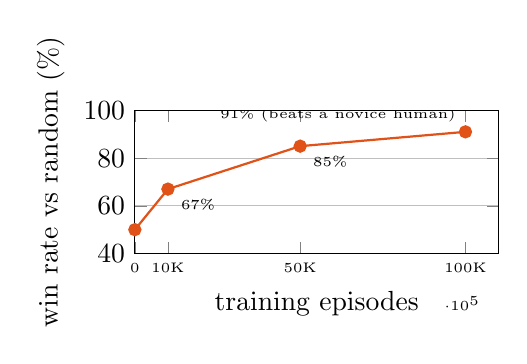
\begin{tikzpicture}\begin{axis}[width=6.2cm,height=3.4cm,xlabel={training episodes},ylabel={win rate vs random (\%)},xmin=0,xmax=110000,ymin=40,ymax=100,xtick={0,10000,50000,100000},xticklabels={0,10K,50K,100K},ymajorgrids,xticklabel style={font=\tiny}]
\addplot[AccentCol,thick,mark=*]coordinates{(0,50)(10000,67)(50000,85)(100000,91)};
\node[font=\tiny,anchor=north west]at(axis cs:11000,67){67\%};\node[font=\tiny,anchor=north west]at(axis cs:51000,85){85\%};\node[font=\tiny,anchor=south east]at(axis cs:100000,91){91\% (beats a novice human)};
\end{axis}\end{tikzpicture}}
\begin{ibox}\scriptsize No labels, no examples of ``the right move'': the agent discovers tactics purely from interaction, exactly like a trainee learning from exercises.\end{ibox}
\end{columns}
\end{frame}

\begin{frame}{Reinforcement Learning --- Bellman Equation, Q-Learning and DQN}
\begin{columns}[T]
\column{0.52\textwidth}
\begin{fbx}{Bellman optimality equation}\[Q^{*}(s,a)=\sum_{s'}P(s'|s,a)\Big[R+\gamma\max_{a'}Q^{*}(s',a')\Big]\]\end{fbx}
\begin{fbx}{Q-learning update rule}\[Q(s,a)\leftarrow Q(s,a)+\alpha\big[r+\gamma\max_{a'}Q(s',a')-Q(s,a)\big]\]\end{fbx}
\begin{tl}\item $\alpha$ = learning rate; $\varepsilon$-greedy: explore with probability $\varepsilon$, exploit with $1-\varepsilon$
\item \textbf{Deep Q-Network (DQN):} replace the Q-table with a neural network $Q(s,a;\theta)\approx Q^{*}(s,a)$ --- handles huge state spaces\end{tl}
\figc{2.0cm}{\begin{tikzpicture}[x=0.8cm,y=0.8cm]
\foreach \i in {0,...,3}{\foreach \j in {0,...,2}{\draw[ISSAgrey,fill=white](\i,\j)rectangle++(1,1);}}
\fill[ISSAgrn!30](3,2)rectangle++(1,1);\node[font=\scriptsize\bfseries]at(3.5,2.5){+100};\fill[ISSAred!25](3,1)rectangle++(1,1);\node[font=\scriptsize\bfseries]at(3.5,1.5){$-100$};\fill[ISSAgrey!50](1,1)rectangle++(1,1);
\node[ndN,inner sep=1pt,minimum height=0.3cm]at(0.5,0.5){S};
\draw[arrA](0.5,0.5)--(0.5,1.4);\draw[arrA](0.5,1.5)--(0.5,2.4);\draw[arrA](0.6,2.5)--(1.4,2.5);\draw[arrA](1.5,2.5)--(2.4,2.5);\draw[arrA](2.5,2.5)--(3.3,2.5);
\node[lab,anchor=west]at(4.2,1.5){learned greedy\\policy $\pi^{*}$\\(follow arrows)};
\end{tikzpicture}}
\column{0.46\textwidth}
\figc{2.9cm}{\begin{tikzpicture}
\node[nd](s)at(0,0){state $s$\\(grid, units)};\node[ndN,minimum width=1.6cm,minimum height=1.4cm](n)at(2.3,0){Neural\\network\\$\theta$};
\node[nds](q1)at(4.5,0.9){$Q(s,\text{move})$};\node[nds](q2)at(4.5,0.3){$Q(s,\text{attack})$};\node[nds](q3)at(4.5,-0.3){$Q(s,\text{defend})$};\node[nds](q4)at(4.5,-0.9){$Q(s,\text{resupply})$};
\draw[arr](s)--(n);\foreach \q in {q1,q2,q3,q4}{\draw[arr](n)--(\q);}
\node[lab]at(2.3,-1.5){DQN: one forward pass gives the value of every action};
\end{tikzpicture}}
\begin{cbox}[ISSAgrn]{Convergence on the wargame (vs random OPFOR)}\scriptsize 10K episodes: \textbf{67\%} win rate; 50K episodes: \textbf{85\%}; 100K episodes: \textbf{91\%} (beats a novice human).\end{cbox}
\begin{ibox}\scriptsize\textbf{Reading the update:} the bracket is the TD error --- the gap between what we predicted ($Q$) and what we then observed ($r+\gamma\max Q'$). Each step nudges $Q$ toward the better estimate. Lectures 6--8 develop this in depth.\end{ibox}
\end{columns}
\end{frame}

\sect{10. Deep Learning}
\begin{frame}{Deep Learning --- Neural Networks \& the Neuron}
\begin{columns}[T]
\column{0.50\textwidth}
\subhead{A single neuron and the network it builds}
\figc{2.3cm}{\begin{tikzpicture}
\foreach \y/\l in {0.9/x_1,0.3/x_2,-0.3/x_3,-0.9/x_i}{\node[font=\scriptsize](x\l)at(0,\y){$\l$};}
\node[circle,draw=ISSAnavy,fill=ISSAlblue!50,minimum size=1cm,font=\scriptsize](n)at(2.3,0){$\sum+b$};\node[circle,draw=ISSAnavy,fill=AccentCol!20,minimum size=0.8cm,font=\scriptsize](a)at(3.9,0){$\sigma$};\node[font=\scriptsize](o)at(5.1,0){$a_j$};
\foreach \l in {x_1,x_2,x_3,x_i}{\draw[arr](x\l)--(n);}\node[lab]at(1.1,1.1){weights $w_{ij}$};\draw[arr](n)--(a);\draw[arr](a)--(o);
\end{tikzpicture}}
\begin{fbx}{Neuron, gradient and update}\[a_j=\sigma\Big(\sum_i w_{ij}x_i+b_j\Big)\]\[\frac{\partial\mathcal{L}}{\partial w_{ij}}=\frac{\partial\mathcal{L}}{\partial a_j}\,\sigma'(z_j)\,x_i,\qquad\theta\leftarrow\theta-\alpha\nabla_\theta\mathcal{L}\]\end{fbx}
\begin{cbox}[ISSAnavy]{Universal approximation (Hornik 1989)}\scriptsize A network with $\ge1$ hidden layer can approximate any continuous function to arbitrary accuracy --- the theoretical foundation of DL.\end{cbox}
\column{0.48\textwidth}
\subhead{Activation functions $\sigma$}
\figc{3.0cm}{\begin{tikzpicture}\begin{axis}[width=6.4cm,height=3.4cm,xmin=-4,xmax=4,ymin=-1.3,ymax=2.2,xlabel={$x$},legend pos=north west,legend columns=2,axis lines=middle,xlabel style={at={(1,0)},anchor=north west}]
\addplot[ISSAblue,thick,domain=-4:4,samples=40]{max(0,x)};\addlegendentry{ReLU}
\addplot[AccentCol,thick,domain=-4:4,samples=60]{1/(1+exp(-x))};\addlegendentry{Sigmoid}
\addplot[ISSAgrn,thick,domain=-4:4,samples=60]{tanh(x)};\addlegendentry{Tanh}
\end{axis}\end{tikzpicture}}
\begin{tl}\item \textbf{ReLU} $\max(0,x)$ --- most common\item \textbf{Sigmoid} $1/(1+e^{-x})$ --- binary output\item \textbf{Softmax} $e^{x_i}/\sum_j e^{x_j}$ --- multi-class\item \textbf{Tanh} $(e^x-e^{-x})/(e^x+e^{-x})$\end{tl}
\end{columns}
\end{frame}

\begin{frame}{Deep Learning --- Why ``Deep''? Hierarchical Features \& Architectures}
\begin{columns}[T]
\column{0.50\textwidth}
\subhead{SAR / satellite image: what each layer learns}
\figc{4.4cm}{\begin{tikzpicture}
\tikzset{Lr/.style={nd,text width=3.3cm,align=left,minimum height=0.5cm,font=\fontsize{6.2}{7}\selectfont}}
\node[Lr,fill=ISSAblue!8]at(0,-0.62){\textbf{L1} pixel edges; shadow boundaries};
\node[Lr,fill=ISSAblue!16]at(0,-1.24){\textbf{L2} corner reflectors; geometric shapes};
\node[Lr,fill=ISSAgrn!14]at(0,-1.86){\textbf{L3} vehicle silhouettes; track marks};
\node[Lr,fill=ISSAgrn!24]at(0,-2.48){\textbf{L4} tank vs APC vs truck type};
\node[Lr,fill=AccentCol!18]at(0,-3.10){\textbf{L5} tactical formation; posture};
\node[Lr,fill=AccentCol!30]at(0,-3.72){\textbf{L6+} context; intent inference};
\draw[bigarr](2.3,-0.4)--(2.3,-3.9);\node[lab,rotate=-90]at(2.75,-2.2){more abstract};
\node[lab,anchor=west]at(2.9,-0.7){shallow (1 layer):\\simple linear\\boundaries};\node[lab,anchor=west]at(2.9,-3.3){deep (5--100+):\\hierarchical\\abstraction};
\end{tikzpicture}}
\begin{ibox}\scriptsize\textbf{Scale law (Kaplan 2020):} more data + more parameters + more compute $\Rightarrow$ better performance, \emph{predictably}.\end{ibox}
\column{0.48\textwidth}
\subhead{Architectures and defence workhorses}
\begin{cbox}[ISSAnavy]{Which architecture for which data?}
{\fontsize{6.3}{7.5}\selectfont\renewcommand{\arraystretch}{1.25}\begin{tabular}{@{}p{1.1cm}p{2.2cm}p{1.8cm}@{}}\toprule\textbf{Net}&\textbf{Data}&\textbf{Result}\\\midrule CNN&Images, SAR, satellite&97.2\% target ID\\RNN/LSTM&Radar tracks, SIGINT&78\% intent prediction\\Transformer&Intel reports, LLMs&88\% NER on SIGINT\\GAN&Synthetic training data&8$\times$ data augmentation\\\bottomrule\end{tabular}}
\end{cbox}
\figc{2.3cm}{\begin{tikzpicture}
\foreach \xx/\nn in {0/3,1.3/5,2.6/5,3.9/2}{\foreach \ii in {1,...,\nn}{\node[circle,draw=ISSAnavy,fill=ISSAlblue!50,inner sep=1.4pt]at(\xx,{(\ii-(\nn+1)/2)*0.4}){};}}
\foreach \xa/\na/\xb/\nb in {0/3/1.3/5,1.3/5/2.6/5,2.6/5/3.9/2}{\foreach \ii in {1,...,\na}{\foreach \jj in {1,...,\nb}{\draw[ISSAgrey!60,line width=0.2pt](\xa,{(\ii-(\na+1)/2)*0.4})--(\xb,{(\jj-(\nb+1)/2)*0.4});}}}
\node[lab]at(0,-1.3){input};\node[lab]at(2,-1.3){hidden layers (feature extraction)};\node[lab]at(3.9,-1.3){output};
\end{tikzpicture}}
\end{columns}
\end{frame}

\sect{11. Generative AI}
\begin{frame}{Generative AI --- How Large Language Models Work}
\subhead{LLMs: the Transformer revolution}
\begin{columns}[T]
\column{0.55\textwidth}
\figc{3.2cm}{\begin{tikzpicture}
\node[nds,minimum width=1.7cm](t)at(0,0){tokens\\``Enemy armour moves north''};
\node[ndA,minimum width=1.5cm](em)at(2.3,0){Embedding\\+ position};
\node[ndN,minimum width=1.8cm,minimum height=1.2cm](at)at(4.5,0){Multi-head\\self-attention\\$\times N$ layers};
\node[ndG,minimum width=1.4cm](ff)at(6.6,0){Feed-forward};
\node[nd,minimum width=1.5cm](sm)at(8.6,0){Softmax\\next token};
\draw[arr](t)--(em);\draw[arr](em)--(at);\draw[arr](at)--(ff);\draw[arr](ff)--(sm);
\begin{scope}[shift={(3.3,-2.4)},x=0.45cm,y=0.45cm]
\foreach \r/\a/\b/\c/\d/\e in {0/9/2/1/1/1,1/3/7/3/1/0,2/1/3/8/2/1,3/1/1/2/9/3,4/0/1/1/4/9}{\foreach \cc/\v in {0/\a,1/\b,2/\c,3/\d,4/\e}{\node[fill=AccentCol!\v0!white,minimum size=0.43cm,inner sep=0pt]at(\cc,-\r){};}}
\node[lab,anchor=east]at(-0.5,-2){query tokens};\node[lab]at(2,0.8){key tokens};\node[lab,anchor=west]at(4.6,-2){attention weights};
\end{scope}
\end{tikzpicture}}
\begin{fbx}{Attention \& pre-training objective}\[\text{Attention}(Q,K,V)=\text{softmax}\!\Big(\tfrac{QK^{\top}}{\sqrt{d_k}}\Big)V\]\[\max_\theta\ P(w_t\mid w_1,\ldots,w_{t-1};\theta)\ \ \text{(next-token prediction)}\]\end{fbx}
\column{0.43\textwidth}
\begin{cbox}[ISSAnavy]{Architecture and scale}\scriptsize Transformer decoder (autoregressive) with multi-head self-attention. \textbf{GPT-3:} 175B parameters, 300B training tokens. \textbf{GPT-4:} $\sim$1.8T parameters (est.), 13T tokens.\end{cbox}
\begin{cbox}[ISSAgrn]{Emergent capabilities at scale}\scriptsize In-context (few-shot) learning $\bullet$ chain-of-thought reasoning $\bullet$ code generation $\bullet$ multi-language.\end{cbox}
\begin{cbox}[violet]{Fine-tuning options}\scriptsize \textbf{Full:} update all $\theta$ (expensive). \textbf{LoRA:} train small adapter matrices (efficient). \textbf{RLHF:} align to human preferences (safety).\end{cbox}
\end{columns}
\end{frame}

\begin{frame}{Generative AI --- LLMs in Defence: Applications and Risks}
\begin{columns}[T]
\column{0.50\textwidth}
\subhead{Defence applications}
\figc{2.0cm}{\begin{tikzpicture}\node[ndN,minimum width=1.8cm,minimum height=1.3cm](l)at(0,0){\textbf{LLM}\\\sm{local, audited}};
\node[ndG,minimum width=2.4cm](a)at(3.4,1.0){Intel synthesis};\node[ndG,minimum width=2.4cm](b)at(3.4,0.35){Threat narration};\node[ndG,minimum width=2.4cm](c)at(3.4,-0.3){COA generation};\node[ndG,minimum width=2.4cm](d)at(3.4,-0.95){Cyber defence};
\foreach \q in {a,b,c,d}{\draw[arr](l)--(\q);}\end{tikzpicture}}
\begin{tl}\item \textbf{Intelligence synthesis:} auto-summarise 500+ daily SIGINT reports into a commander-ready brief in $<2$ minutes
\item \textbf{Threat narration:} convert structured sensor output into a natural-language threat assessment
\item \textbf{COA generation:} suggest courses of action from doctrine + current situation
\item \textbf{Cyber defence:} analyse malware code, generate YARA rules, explain CVEs to non-technical commanders\end{tl}
\column{0.48\textwidth}
\subhead{Risks in defence}
\figc{2.0cm}{\bars{10}{1.4}{1.5}{Hallucination/9/ISSAred,Poisoning/7/ISSAamb,No interpretability/8/ISSAred,Latency 2--15 s/6/ISSAamb,Data leakage/9/ISSAred}}
\sm{Illustrative qualitative severity for defence use (not measured data)}
\begin{wbox}\scriptsize\textbf{LLM RISKS IN DEFENCE}\begin{tl}\item \textbf{Hallucination:} confident but WRONG facts --- dangerous in battle planning
\item \textbf{Data poisoning:} adversarially manipulated pre-training data
\item \textbf{No interpretability:} why did the model recommend this COA?
\item \textbf{Latency:} GPT-4 API 2--15 s: unacceptable for real-time tactical decisions
\item \textbf{Classified leakage:} cloud LLMs unsuitable for sensitive operations\end{tl}\end{wbox}
\end{columns}
\end{frame}

\begin{frame}{Retrieval Augmented Generation (RAG) for Defence Intelligence}
\subhead{RAG: grounding LLMs in verified, classified knowledge}
\figc{1.6cm}{\begin{tikzpicture}
\node[ndY,minimum width=3cm,minimum height=1.1cm](q)at(0,0){\textbf{QUERY}\\\sm{``Capability of Type-99A MBT in mountain terrain ops?''}};
\node[ndA,minimum width=3cm,minimum height=1.1cm](r)at(3.7,0){\textbf{RETRIEVE}\\\sm{vector-DB search over doctrine + OSINT $\to$ top-5 chunks}};
\node[ndN,minimum width=3cm,minimum height=1.1cm](g)at(7.4,0){\textbf{AUGMENT}\\\sm{query + retrieved context $\to$ LLM prompt}};
\node[ndG,minimum width=3cm,minimum height=1.1cm](o)at(11.1,0){\textbf{GENERATE}\\\sm{answer with source doc IDs: auditable}};
\draw[bigarr](q)--(r);\draw[bigarr](r)--(g);\draw[bigarr](g)--(o);
\end{tikzpicture}}
\begin{columns}[T]
\column{0.48\textwidth}
\figc{2.7cm}{\begin{tikzpicture}\begin{axis}[ybar,width=7.0cm,height=3.5cm,symbolic x coords={Factual accuracy,Hallucination rate,Source citability},xtick=data,ymin=0,ymax=110,bar width=11pt,enlarge x limits=0.25,ylabel={\%},legend style={at={(0.98,0.98)},anchor=north east},nodes near coords,nodes near coords style={font=\fontsize{5}{6}\selectfont},ymajorgrids]
\addplot[fill=ISSAred!60]coordinates{(Factual accuracy,73.2)(Hallucination rate,18.4)(Source citability,0)};\addlegendentry{Bare LLM}
\addplot[fill=ISSAgrn!70]coordinates{(Factual accuracy,94.6)(Hallucination rate,3.2)(Source citability,91.8)};\addlegendentry{RAG-enabled}
\end{axis}\end{tikzpicture}}
\begin{rbox}\scriptsize\textbf{Trade-off:} RAG costs about $+1.3$ s latency (2.1 s $\to$ 3.4 s) and $+\$0.02$ per query ($\$0.04\to\$0.06$) for a \textbf{+21.4\%} accuracy gain and near-zero hallucination.\end{rbox}
\column{0.50\textwidth}
\begin{cbox}[ISSAnavy]{Secure defence RAG architecture}
\figc{2.5cm}{\begin{tikzpicture}
\draw[dashed,ISSAred,rounded corners=3pt](-0.3,-1.7)rectangle(6.3,1.2);\node[lab,ISSAred,anchor=north west]at(-0.2,1.2){air-gapped on-premise zone};
\node[nds](kb)at(1.0,0.5){Knowledge base\\doctrine + manuals};\node[nds](em)at(3.2,0.5){Embedding model\\(BERT, defence corpus)};\node[nds](vs)at(5.3,0.5){Vector store\\FAISS / Chroma};
\node[nds,minimum width=2.2cm](llm)at(3.2,-0.8){Local LLM: Llama-3-70B / Mistral\\on secure GPU server};\node[nds](sec)at(0.9,-0.9){Encrypted at rest\\query logs monitored\\access control};
\draw[arr](kb)--(em);\draw[arr](em)--(vs);\draw[arr](vs)--(llm);\draw[arr](sec)--(llm);
\end{tikzpicture}}
\scriptsize No cloud dependency for classified data.
\end{cbox}
\end{columns}
\end{frame}

\sect{12. Defence Apps}
\begin{frame}{AI/ML in Defence --- Application Landscape}
\subhead{Comprehensive AI/ML application map for defence \& wargaming}
\figc{4.6cm}{\begin{tikzpicture}
\tikzset{D/.style={nd,text width=3.6cm,align=left,minimum height=1.45cm,font=\fontsize{6}{7.2}\selectfont,inner sep=3pt}}
\node[D,draw=ISSAblue,fill=ISSAblue!8](a)at(-4.1,1.2){\textbf{ISR}\\$\bullet$ SAR/EO image analysis (CNN)\\$\bullet$ SIGINT pattern recog. (LSTM)\\$\bullet$ Multi-source fusion (Transformer)\\$\bullet$ HUMINT synthesis (LLM)};
\node[D,draw=ISSAred,fill=ISSAred!6](b)at(0,1.2){\textbf{CYBER OPS}\\$\bullet$ Intrusion detection (unsup.)\\$\bullet$ Malware classification (RF)\\$\bullet$ APT clustering (DBSCAN)\\$\bullet$ Vulnerability assessment (DL)};
\node[D,draw=ISSAgrn,fill=ISSAgrn!8](c)at(4.1,1.2){\textbf{AUTONOMOUS SYSTEMS}\\$\bullet$ UAV path planning (RL+A*)\\$\bullet$ Swarm coordination (MARL)\\$\bullet$ Mine detection (CNN+fusion)\\$\bullet$ Autonomous vehicles (SLAM)};
\node[D,draw=ISSAamb,fill=ISSAyell!50](d)at(-4.1,-1.2){\textbf{LOGISTICS}\\$\bullet$ Demand forecast (LSTM/ARIMA)\\$\bullet$ Predictive maintenance (XGBoost)\\$\bullet$ Route optimisation (RL)\\$\bullet$ Fuel modelling (linear reg.)};
\node[D,draw=violet,fill=violet!8](e)at(0,-1.2){\textbf{WARGAMING \& SIMULATION}\\$\bullet$ OPFOR agents (DQN/PPO)\\$\bullet$ Terrain analysis (CNN+GIS)\\$\bullet$ Attrition modelling (SVM/NN)\\$\bullet$ COA generation (LLM+RL)};
\node[D,draw=AccentCol,fill=AccentCol!8](f)at(4.1,-1.2){\textbf{C2 \& DECISION SUPPORT}\\$\bullet$ Battlefield visualisation (DL)\\$\bullet$ Force tracking (Kalman+ML)\\$\bullet$ Commander briefing (RAG+LLM)\\$\bullet$ Info-overload filter (NLP)};
\draw[arr,<->,ISSAgrey](a)--(b);\draw[arr,<->,ISSAgrey](b)--(c);\draw[arr,<->,ISSAgrey](d)--(e);\draw[arr,<->,ISSAgrey](e)--(f);\draw[arr,<->,ISSAgrey](a)--(d);\draw[arr,<->,ISSAgrey](b)--(e);\draw[arr,<->,ISSAgrey](c)--(f);
\end{tikzpicture}}
\begin{ibox}\scriptsize\textbf{India defence AI:} DRDO AI-enabled artillery fire control, ISRO ML-based satellite image analysis, Navy sonar ML systems, Army autonomous surveillance UGVs --- active deployments across all six domains. Data flows ISR $\to$ C2 $\to$ Wargaming $\to$ Autonomous Systems in the sensor-to-shooter chain.\end{ibox}
\end{frame}

\sect{13. Wargaming Cases}
\begin{frame}{AI in Wargaming --- Computer Generated Forces and Attrition Modelling}
\begin{columns}[T]
\column{0.50\textwidth}
\subhead{Computer Generated Forces (CGF)}
\figc{1.7cm}{\begin{tikzpicture}\node[ndR,text width=2.6cm](x)at(0,0){\textbf{Traditional:} scripted NPC behaviour --- predictable, exploitable};\node[ndG,text width=3.4cm](y)at(4.3,0){\textbf{AI-enhanced OPFOR:} adaptive, doctrine-adherent RL agents};\draw[bigarr](x)--(y);\end{tikzpicture}}
\begin{tl}\item Multi-echelon: strategic $\to$ operational $\to$ tactical; adapts mid-exercise to Blue strategy
\item DRL OPFOR effectiveness: \textbf{78\%} of an expert human; cost $\sim$1/1000th of human OPFOR staffing; available 24/7\end{tl}
\column{0.48\textwidth}
\subhead{Attrition: Lanchester's laws, enhanced by ML}
\figc{2.5cm}{\bars{1}{1.8}{2.4}{Classical Lanchester $R^2$/0.61/ISSAred,RF with terrain + weather + morale + EW $R^2$/0.87/ISSAgrn}}
\begin{fbx}{Classical Lanchester}\[\tfrac{dR}{dt}=-\alpha B,\qquad\tfrac{dB}{dt}=-\beta R\]\end{fbx}
\sm{Random Forest evaluated on 1,200 engagements.}
\end{columns}
\end{frame}

\begin{frame}{AI in Wargaming --- Terrain, COA Generation and Maturity Levels}
\begin{columns}[T]
\column{0.50\textwidth}
\subhead{Terrain \& COA analysis with AI}
\figc{2.5cm}{\bars{100}{1.8}{1.6}{Terrain CNN accuracy/94.8/ISSAgrn,AI COAs rated acceptable/72/ISSAamb,Staff COAs rated acceptable/89/ISSAblue}}
\begin{tl}\item \textbf{Terrain (ResNet-34):} 50K patches (1 km$^2$), 5 classes; 94.8\%, 11 ms/patch. Manual GIS 4 h per 1000 km$^2$ vs AI 12 min ($20\times$)
\item \textbf{COA (LLM+RL):} MDMP planning cycle 6 h vs AI: 3 options in 45 s; quality gap 17 points $\Rightarrow$ initial planning support, not final orders\end{tl}
\column{0.48\textwidth}
\subhead{Wargame AI maturity levels}
\figc{3.0cm}{\begin{tikzpicture}
\foreach \i/\t/\c in {1/L1 Scripted AI (current standard)/ISSAblue!15,2/L2 Adaptive RL agents (emerging)/ISSAblue!28,3/L3 Multi-agent coalition tactics (research)/ISSAgrn!25,4/L4 Strategic AI advisors with LLM reasoning (near-future)/AccentCol!25,5/L5 Autonomous campaign planning (far-future)/AccentCol!45}{\node[anchor=west,draw=ISSAnavy,fill=\c,minimum height=0.46cm,minimum width={1.6cm+\i*0.9cm},font=\fontsize{5.8}{6.5}\selectfont,inner sep=2pt]at(0,\i*0.5){\t};}
\end{tikzpicture}}
\begin{wbox}\scriptsize\textbf{SIMULATION-TO-REALITY GAP:} a 91\% win rate in JANUS $\neq$ 91\% real-world performance. Sim-to-real transfer, fog of war, adversarial adaptation and friction must be modelled explicitly. Over-confidence in wargame AI results is a known failure mode.\end{wbox}
\end{columns}
\end{frame}

\sect{14. Data Pitfalls}
\begin{frame}{Data Pitfalls --- Why Bad Data Produces Dangerous AI}
\subhead{The six critical data pitfalls in defence AI (overview)}
\figc{4.1cm}{\begin{tikzpicture}
\tikzset{H/.style={nd,text width=3.5cm,align=left,minimum height=1.55cm,font=\fontsize{6.2}{7.4}\selectfont,inner sep=3pt,draw=ISSAred,fill=ISSAred!5}}
\node[H](a)at(-3.9,0.9){\textbf{1  SURVIVORSHIP BIAS}\\Study only survivors $\to$ ignore failures.\\\textit{Ex: train only on won battles}};
\node[H](b)at(0,0.9){\textbf{2  SPURIOUS CORRELATION}\\Correlation $\neq$ causation.\\\textit{Ex: ``lunch quality'' predicts exercise wins?}};
\node[H](c)at(3.9,0.9){\textbf{3  OVERFITTING \& DIST. SHIFT}\\Model memorises data; fails in a new environment.\\\textit{Ex: Afghan terrain $\to$ Iraq}};
\node[H](d)at(-3.9,-1.0){\textbf{4  TRAINING DATA BIAS}\\Skewed training set; class imbalance; confirmation bias in labels.};
\node[H](e)at(0,-1.0){\textbf{5  LABEL NOISE}\\5\% noise $\to$ $-3.4\%$ acc.; 30\% $\to$ $-35\%$.\\Adversarial poisoning possible.};
\node[H](f)at(3.9,-1.0){\textbf{6  MISUSE OF STATISTICS}\\P-hacking, cherry-picking; mean without context; Simpson's paradox.};
\end{tikzpicture}}
\begin{columns}[T]
\column{0.50\textwidth}
\begin{cbox}[ISSAnavy]{Reference thread}\scriptsize AK Dhamija (SlideShare: Goody Research --- Compatibility Mode) presents fundamental flaws in using data and drawing incorrect conclusions from research. The slides that follow extend these ideas with defence examples and AI-specific failures.\end{cbox}
\column{0.48\textwidth}
\begin{wbox}\scriptsize\textbf{Mark Twain:} ``There are three kinds of lies: lies, damned lies, and statistics.'' In defence AI the stakes are existential: a mis-trained model advising a commander is an operational liability.\end{wbox}
\end{columns}
\end{frame}

\begin{frame}{Data Pitfall \#1 --- Survivorship Bias: Studying Only the Winners}
\begin{columns}[T]
\column{0.50\textwidth}
\subhead{The classic case: Wald \& WWII bombers (1943)}
\figc{3.5cm}{\begin{tikzpicture}
\draw[fill=ISSAgrey!30,rounded corners=7pt](-0.28,-2.0)rectangle(0.28,2.0);
\draw[fill=ISSAgrey!30](-0.28,0.7)--(-2.8,-0.5)--(-2.8,-1.05)--(-0.28,-0.25)--cycle;\draw[fill=ISSAgrey!30](0.28,0.7)--(2.8,-0.5)--(2.8,-1.05)--(0.28,-0.25)--cycle;
\draw[fill=ISSAgrey!30](-0.28,-1.55)--(-1.1,-2.0)--(-1.1,-2.3)--(-0.28,-1.95)--cycle;\draw[fill=ISSAgrey!30](0.28,-1.55)--(1.1,-2.0)--(1.1,-2.3)--(0.28,-1.95)--cycle;
\foreach \x/\y in {-2.2/-0.55,-1.9/-0.8,-2.6/-0.8,2.1/-0.6,1.7/-0.4,2.5/-0.85,0.1/0.2,-0.1/-0.6,0.12/-1.0,-0.8/-2.1,0.9/-2.15,0.05/-1.4}{\fill[ISSAred](\x,\y)circle(0.06);}
\draw[ISSAgrn,dashed,line width=1pt](-1.15,0.05)circle(0.22);\draw[ISSAgrn,dashed,line width=1pt](1.15,0.05)circle(0.22);\draw[ISSAgrn,dashed,line width=1pt](0,1.55)circle(0.3);
\node[lab,ISSAgrn,anchor=west]at(1.4,1.1){engines \& cockpit: NO holes seen\\$\Rightarrow$ these hits are fatal};\node[lab,ISSAred,anchor=west]at(1.4,-1.5){\textbullet\ holes on returning aircraft};
\end{tikzpicture}}
\begin{tl}\item USAF analysed returning B-17s: wings \& fuselage most shot up $\Rightarrow$ ``armour those areas!''
\item \textbf{Wald's correction:} you only see planes that \emph{returned}. Planes hit in the engines/cockpit are at the bottom of the ocean --- armour where you see \textbf{no} damage.\end{tl}
\column{0.48\textwidth}
\subhead{Wargaming AI application}
\figc{2.1cm}{\bars{100}{1.5}{2.0}{Biased model: predicted win rate/74/ISSAred,Actual exercise win rate/53/ISSAgrn}}
\begin{wbox}\scriptsize Training only on battles survived/won predicted \textbf{74\%} vs an actual \textbf{53\%}: over-estimation of $+39.6\%$ --- catastrophic. \textbf{Fix:} seek defeat records, OPFOR after-action reports and classified failure analyses; weight rare failures appropriately.\end{wbox}
\begin{cbox}[ISSAnavy]{Other military examples}\scriptsize Equipment reliability: failed units are destroyed, so data shows survivors only. Doctrine analysis: operations written up only if successful. Fund rankings: only surviving funds appear.\end{cbox}
\begin{ibox}\scriptsize\textbf{RED FLAG:} if a dataset contains ONLY successes, your model is optimistic by design --- ask ``Where are the failure records?''\end{ibox}
\end{columns}
\end{frame}

\begin{frame}{Data Pitfall \#2 --- Spurious Correlation \& Simpson's Paradox}
\begin{columns}[T]
\column{0.50\textwidth}
\subhead{Correlation $\neq$ causation}
\figc{2.1cm}{\begin{tikzpicture}\node[ndY](t)at(2.2,1.2){Summer heat\\\sm{CONFOUNDER}};\node[nd](i)at(0,0){Ice-cream sales};\node[nd](s)at(4.4,0){Shark attacks};
\draw[arr](t)--(i);\draw[arr](t)--(s);\draw[arr,dashed,ISSAred,<->](i)--node[above,lab]{$r=0.92$ (spurious!)}(s);\end{tikzpicture}}
\begin{cbox}[ISSAred]{Defence example (3 years of wargame data)}\scriptsize ``Catering quality survey'' correlates with exercise win rate, $r=0.71$. Confounder: budget/readiness. Controlling for budget: $r_{\text{partial}}=0.09$ ($p=0.42$) --- the effect vanishes.\end{cbox}
\begin{cbox}[ISSAnavy]{Simpson's paradox}\scriptsize A trend that appears in every subgroup can \textbf{reverse} in the combined data when group sizes are unequal.\end{cbox}
\column{0.48\textwidth}
\subhead{Simpson's paradox: always show the counts}
\figc{2.2cm}{\scriptsize\renewcommand{\arraystretch}{1.2}\begin{tabular}{lcc}\toprule&\textbf{Treatment A}&\textbf{Treatment B}\\\midrule Small stones&81/87 = 93\%&234/270 = 87\%\\Large stones&192/263 = 73\%&55/80 = 69\%\\\midrule Combined&273/350 = \textbf{78\%}&289/350 = \textbf{83\%}\\\bottomrule\end{tabular}}
\begin{ibox}\scriptsize A wins in \emph{both} subgroups but loses overall: A treated mostly the hard (large-stone) cases. Percentages cannot be added or averaged --- totals must come from the counts (see Section 0).\end{ibox}
\begin{rbox}\scriptsize Wargame twin: AI-assisted units 186/300 = 62\% vs conventional 256/320 = 80\% overall, yet AI units win more in every terrain.\end{rbox}
\end{columns}
\end{frame}

\begin{frame}{Data Pitfall \#2 (cont.) --- Misuse of Statistics \& Shortcut Learning}
\subhead{Statistics as a weapon (against you): five key flaws}
\begin{columns}[T]
\column{0.58\textwidth}
\figc{3.9cm}{\begin{tikzpicture}
\tikzset{S/.style={nd,text width=7.2cm,align=left,minimum height=0.7cm,font=\fontsize{6.4}{7.6}\selectfont,inner sep=3pt,draw=ISSAamb,fill=ISSAyell!40}}
\node[S]at(0,0){\textbf{1 MEAN WITHOUT CONTEXT.} Average soldier salary Rs 35K/month but median Rs 22K (few senior officers skew the mean) --- report median + IQR.};
\node[S]at(0,-0.85){\textbf{2 P-HACKING.} Run 20 tests at $p<0.05$: expect 1 false positive by chance; $p=0.048$ means little if 50 other tests were run first.};
\node[S]at(0,-1.7){\textbf{3 CHERRY-PICKING.} Reporting only the windows/subgroups that confirm the hypothesis. Full reporting required.};
\node[S]at(0,-2.55){\textbf{4 SMALL-SAMPLE OVERGENERALISATION.} 3 wargame exercises $\to$ ``AI always outperforms''. Need $N\ge30$ for basic CLT guarantees.};
\node[S]at(0,-3.4){\textbf{5 ECOLOGICAL FALLACY.} Group-level pattern $\neq$ individual-level: ``brigades with more AI tools win more'' does not mean a specific brigade will.};
\end{tikzpicture}}
\column{0.40\textwidth}
\figc{1.8cm}{\begin{tikzpicture}[x=0.8cm,y=0.5cm]
\draw[->](0,0)--(5.2,0);\draw[ISSAblue,fill=ISSAblue!20](0,0)..controls(0.8,0)and(0.9,3)..(1.4,3)..controls(2.0,3)and(2.0,0.8)..(3.0,0.4)..controls(4,0.15)and(4.6,0.1)..(5,0.0)--cycle;
\draw[ISSAgrn,thick](1.45,0)--(1.45,3.4);\node[lab,ISSAgrn,anchor=south]at(1.45,3.4){median};\draw[ISSAred,thick](2.5,0)--(2.5,3.4);\node[lab,ISSAred,anchor=south]at(2.5,3.4){mean};
\end{tikzpicture}}
\begin{wbox}\scriptsize\textbf{SHORTCUT LEARNING (AI-specific):} a CNN classifying tanks learned the \emph{background} (blue sky in the training photos), not the tank. In wargaming: a model infers ``night operations'' from timestamp metadata rather than thermal signatures --- an adversary can exploit this.\end{wbox}
\figc{1.5cm}{\begin{tikzpicture}\node[nds,fill=ISSAlblue!50](a)at(0,0){train: tank + sky};\node[nds,fill=ISSAlblue!50](b)at(0,-0.7){train: no tank + cloud};\node[ndR](c)at(2.9,-0.35){model keys on sky};\draw[arr](a)--(c);\draw[arr](b)--(c);\end{tikzpicture}}
\end{columns}
\end{frame}

\begin{frame}{Data Pitfall \#3 --- Overfitting: the Mine Detection Systems}
\begin{columns}[T]
\column{0.48\textwidth}
\subhead{Error vs model complexity}
\figc{3.2cm}{\begin{tikzpicture}\begin{axis}[width=6.6cm,height=3.8cm,xlabel={model complexity},ylabel={error},xmin=0,xmax=10,ymin=0,ymax=1,ticks=none,legend pos=north east]
\addplot[ISSAblue,thick,domain=0.4:10,samples=40]{0.9*exp(-0.45*x)+0.04};\addlegendentry{train}
\addplot[AccentCol,thick,domain=0.4:10,samples=40]{0.9*exp(-0.55*x)+0.1+0.012*x^2};\addlegendentry{test}
\draw[dashed,ISSAgrey](axis cs:3.4,0)--(axis cs:3.4,1);\node[font=\tiny,anchor=south west]at(axis cs:3.5,0.02){sweet spot};\node[font=\tiny,ISSAred]at(axis cs:8.2,0.5){overfit};\node[font=\tiny,ISSAblue]at(axis cs:0.9,0.95){underfit};
\end{axis}\end{tikzpicture}}
\begin{cbox}[ISSAnavy]{Mine detection (GPR + metal detector)}\scriptsize 800 samples, Afghan terrain, 47 signal features. \textbf{Model A:} simple CNN, 200K params. \textbf{Model B:} deep ResNet, 25M params.\end{cbox}
\column{0.50\textwidth}
\subhead{Accuracy by test domain (\%)}
\figc{3.2cm}{\begin{tikzpicture}\begin{axis}[ybar,width=7.0cm,height=3.8cm,symbolic x coords={Train,Test Afghan,Test Iraq},xtick=data,ymin=40,ymax=105,bar width=13pt,enlarge x limits=0.25,legend style={at={(0.5,1.02)},anchor=south,legend columns=2},nodes near coords,nodes near coords style={font=\fontsize{5.5}{6}\selectfont},ymajorgrids]
\addplot[fill=ISSAblue!60]coordinates{(Train,88.4)(Test Afghan,86.2)(Test Iraq,82.7)};\addlegendentry{Model A (simple)}
\addplot[fill=ISSAred!65]coordinates{(Train,97.3)(Test Afghan,94.1)(Test Iraq,58.7)};\addlegendentry{Model B (deep)}
\end{axis}\end{tikzpicture}}
\begin{wbox}\scriptsize Model B overfit to Afghan soil signatures: deployed in Iraq it reached only \textbf{58.7\%} --- catastrophic. The bigger, better-looking model was the worse fielded system.\end{wbox}
\end{columns}
\end{frame}

\begin{frame}{Data Pitfall \#3 --- Distribution Shift: Detect It Before You Deploy}
\begin{columns}[T]
\column{0.50\textwidth}
\subhead{Train vs deployment input distributions}
\figc{2.4cm}{\begin{tikzpicture}\begin{axis}[width=6.4cm,height=3.0cm,xlabel={input feature $x$},ylabel={density},ticks=none,domain=-4:8,samples=60,legend pos=north east]
\addplot[ISSAblue,thick,fill=ISSAblue!20]{exp(-x^2/2)/2.5};\addlegendentry{training (Afghanistan)}
\addplot[ISSAred,thick,fill=ISSAred!15,fill opacity=0.6]{exp(-(x-3.2)^2/3)/2.5};\addlegendentry{deployment (Iraq)}
\end{axis}\end{tikzpicture}}
\begin{fbx}{Kolmogorov--Smirnov shift detector}\[D=\max_x\,\big|F_{\text{new}}(x)-F_{\text{train}}(x)\big|\ \ \Rightarrow\ \text{alert if }D>\tau\]\end{fbx}
\column{0.48\textwidth}
\subhead{Causes and remedies}
\figc{1.9cm}{\begin{tikzpicture}\begin{axis}[width=5.8cm,height=2.6cm,xlabel={$x$},ylabel={CDF},ticks=none,domain=-4:8,samples=50]
\addplot[ISSAblue,thick]{1/(1+exp(-1.7*x))};\addplot[ISSAred,thick]{1/(1+exp(-1.2*(x-3.2)))};
\draw[<->,AccentCol,thick](axis cs:1.6,0.063)--(axis cs:1.6,0.82);\node[font=\tiny,AccentCol,anchor=west]at(axis cs:1.7,0.45){$D$ (KS gap)};
\end{axis}\end{tikzpicture}}
\begin{tl}\item \textbf{Causes:} day vs night imagery; desert vs jungle; 2021 vs 2026 threat profiles
\item \textbf{Remedies:} L2 regularisation, dropout, early stopping, data augmentation, domain-adaptive training\end{tl}
\begin{rbox}\scriptsize\textbf{PROTOCOL:} test on data from the \textbf{deployment} domain, across all anticipated environments, weather and adversary adaptations, \emph{before} fielding.\end{rbox}
\end{columns}
\end{frame}

\begin{frame}{Data Pitfalls \#4 \& \#5 --- Training Data Bias and Label Noise}
\begin{columns}[T]
\column{0.50\textwidth}
\subhead{Label noise impact ($N=10{,}000$ defence sensor samples)}
\figc{3.2cm}{\begin{tikzpicture}\begin{axis}[width=6.6cm,height=3.8cm,xlabel={label noise rate (\%)},ylabel={accuracy (\%)},xmin=0,xmax=32,ymin=50,ymax=100,ymajorgrids]
\addplot[AccentCol,thick,mark=*]coordinates{(0,97.2)(5,93.8)(10,88.1)(20,76.4)(30,61.7)};
\node[font=\tiny,anchor=south west]at(axis cs:0.5,97.5){0\%: 97.2 baseline};\node[font=\tiny,anchor=west]at(axis cs:5.5,94.5){5\%: 93.8 ($-3.4$)};\node[font=\tiny,anchor=west]at(axis cs:10.5,89){10\%: 88.1 ($-9.1$)};\node[font=\tiny,anchor=west]at(axis cs:20.5,77){20\%: 76.4 ($-20.8$)};\node[font=\tiny,anchor=south,ISSAred]at(axis cs:27,62){30\%: 61.7 ($-35.5$) near-useless};
\end{axis}\end{tikzpicture}}
\begin{wbox}\scriptsize\textbf{ADVERSARIAL POISONING:} 3\% poisoning $\to$ 94\% flip on the target class. Training pipelines must be cryptographically signed and anomaly-monitored.\end{wbox}
\column{0.48\textwidth}
\subhead{Training data bias}
\figc{1.6cm}{\begin{tikzpicture}\fill[ISSAblue!70](0,0)rectangle(9.5,0.5);\fill[ISSAred!80](9.5,0)rectangle(10,0.5);\node[white,font=\scriptsize\bfseries]at(4.7,0.25){95\% non-threat};\node[font=\tiny,ISSAred,anchor=south]at(9.75,0.5){5\% threat};\end{tikzpicture}}
\begin{cbox}[ISSAred]{Class imbalance}\scriptsize Training 95\% non-threat / 5\% threat $\to$ model predicts ``non-threat'' always: \textbf{95\% accuracy but ZERO threat detection}. Fix: class weighting, SMOTE oversampling.\end{cbox}
\begin{cbox}[ISSAamb]{Selection bias}\scriptsize Non-representative collection: facial recognition trained on Caucasian faces gave 34\% error on darker skin tones (MIT 2018). Intel labels are biased by the analyst's prior beliefs (confirmation bias).\end{cbox}
\end{columns}
\end{frame}

\sect{15. Summary}
\begin{frame}{Lecture 1 Summary --- Key Takeaways}
\subhead{What we covered today: 15 key points in 6 categories}
\figc{4.5cm}{\begin{tikzpicture}
\tikzset{K/.style={nd,text width=3.6cm,align=left,minimum height=1.8cm,font=\fontsize{6.4}{7.6}\selectfont,inner sep=3pt}}
\node[K,draw=ISSAblue,fill=ISSAblue!8]at(-4,1.1){\textbf{AI FOUNDATIONS}\\AI = making machines mimic cognition. Spans classical (rules) to GenAI (learned). Narrow AI is the current state of the art.};
\node[K,draw=ISSAgrn,fill=ISSAgrn!8]at(0,1.1){\textbf{ML REVOLUTION}\\Learn patterns from DATA, not rules. Enabled by data + GPU compute. Explosion post-2012 (ImageNet/AlexNet).};
\node[K,draw=violet,fill=violet!8]at(4,1.1){\textbf{5 PARADIGMS}\\Supervised / unsupervised / semi-supervised / self-supervised / reinforcement. Each suits a different data-availability scenario.};
\node[K,draw=ISSAamb,fill=ISSAyell!40]at(-4,-1.1){\textbf{DEEP LEARNING}\\Multi-layer NNs: hierarchical features. CNN (images), RNN/LSTM (sequences), Transformer (attention) --- the defence workhorses.};
\node[K,draw=AccentCol,fill=AccentCol!8]at(0,-1.1){\textbf{GENERATIVE AI}\\LLMs predict tokens (Transformer decoder). RAG grounds LLMs in verified sources. Defence: ISR synthesis, COA, cyber analysis.};
\node[K,draw=ISSAred,fill=ISSAred!7]at(4,-1.1){\textbf{6 DATA PITFALLS}\\Survivorship bias $\bullet$ spurious correlation $\bullet$ statistical misuse $\bullet$ overfitting/dist. shift $\bullet$ training bias $\bullet$ label noise/poisoning.};
\end{tikzpicture}}
\end{frame}

\begin{frame}{Looking Ahead --- Lecture 2: Supervised Learning (Classification)}
\begin{columns}[T]
\column{0.48\textwidth}
\subhead{Lecture 2 topics}
\begin{tl}\item Decision-boundary concept\item Logistic regression (classification)\item $k$-Nearest Neighbours (kNN)\item Decision Trees \& the CART algorithm\item Random Forest (ensemble methods)\item Support Vector Machines: hard \& soft margin, kernel trick (RBF, polynomial)\item Naive Bayes classifier\item Evaluation: precision / recall / F1 / ROC-AUC\item Worked numerical examples throughout\end{tl}
\begin{ibox}\scriptsize\textbf{Pre-reading:} matrix operations, probability fundamentals (Bayes' theorem) and the sigmoid function --- Lectures 2--3 use linear-algebra notation extensively.\end{ibox}
\column{0.50\textwidth}
\begin{cbox}{Lecture 2 case study (preview)}\scriptsize \textbf{Multi-class threat classification for IADS:} 5 classes (friendly fighter, adversary bomber, cruise missile, UAV/drone, civilian); 11 features (8 radar + 3 EW); $N=8{,}500$ samples (80/15/5 train/val/test). We will compare \textbf{all} algorithms on the same data: which wins? what trade-offs? is 99\% test accuracy trustworthy? (\emph{Spoiler: distribution shift will strike again!}) All derivations from first principles, with defence-specific numerical context.\end{cbox}
\begin{rbox}\scriptsize\textbf{Assignment 1} (released today, Part 3 of this lecture pack): solve the problems at home; bring written solutions to Lecture 2 --- the first 5 minutes will discuss common errors.\end{rbox}
\end{columns}
\end{frame}
\end{document}
